\documentclass[english,ph, handout]{URbeamer}

\usepackage{babel}
\usepackage[utf8]{inputenc}
\usepackage[T1]{fontenc}
\usepackage{lmodern}
\usepackage{geometry}
\usepackage{graphicx}
\usepackage{amsmath}
\usepackage{multimedia}
\usepackage[ugly]{units}
%\usepackage{placeins}
\usepackage[backend=bibtex, style=numeric-comp, sorting=nty]{biblatex}
\addbibresource{bib.bib}

\newcommand{\diff}{\mathrm{d}}

\setbeameroption{show notes}
\let\orignote\note
%\renewcommand{\note}[1]{\orignote{
%		\begin{minipage}{\textwidth}
%			#1
%		\end{minipage}
%	}}
\renewcommand{\note}[1]{\orignote{\scriptsize{
			#1
			}}}

\title{Evolution of topological surface states of thin HgTe-films with film thickness}
\institute{Fakultät für Physik}
\subtitle{Bachelor thesis}
\author{Tamara Szecsey}

\begin{document}
	\frame[plain]{\titlepage \note{Hello, my name is Tamara Szecsey and I will now give you a talk about my bachelor thesis topic, the evolution of topological surface states of thin HgTe-films with film thickness.}}
	
%	\begin{frame}
%		\maketitle
%%		\begin{figure} [h] 
%%%			\begin{center}
%%%				\includegraphics[width=0.7\textwidth]{n-117451542-large570}
%%%			\end{center}
%%		\end{figure}
%	\end{frame}
	
	\begin{frame}{Table of contents}
		\tableofcontents
	\end{frame}
	
	\section{Introduction}
	\begin{frame}{Introduction}
		HgTe is a II-VI semiconductor and a topological insulator (TI).\footfullcite{top_surf_states}
		\vspace{10px}
	\begin{columns} 
		\begin{column}<2->{0.35\linewidth} \centering
			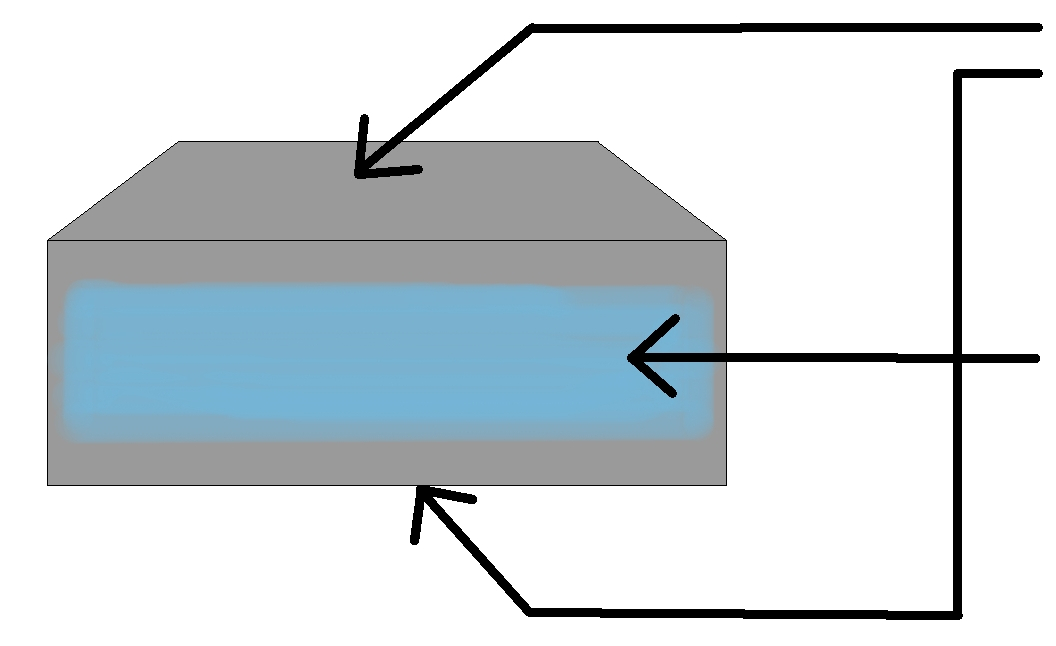
\includegraphics[width=\linewidth]{extrabilder_fuer_vortrag/Introduction1.jpg}
		\end{column}
		\begin{column}<2->{0.23\linewidth} 
			conducting surface states
			
			\vspace{5px}
			insulating in the bulk
			
			\vspace{15pt}
		\end{column}\hfill
		\begin{column}<3->{0.5\linewidth} 
			TIs are interesting because:
			\begin{itemize}
				\item<4-> spin-momentum locking
				\item<5-> protected surface states
			\end{itemize}
		\end{column}\hfill
	\end{columns}
	
	\note{HgTe belongs to the class of mercury-based II-VI semiconductors which appear in zinc-blende structure. It is additionally found to be a topological insulator.\\
	A topological insulator is a material which is insulating in its interior, also called the bulk of a material, and that develops conducting states at the surface.\\
	They are very attractive for potential applications because the spin and the momentum of the electrons at the conducting surfaces are locked. This means, the spin is always perpendicular to the direction of motion of those electrons.
	The spin-momentum locking make sure that the surfaces are protected if time-reversal symmetry preserved. In other words the surface states remain even for non-magnetic impurities.\\}
	\begin{columns}
		\begin{column}<6->{\linewidth}
		Calculations were performed using density functional theory (DFT) through FHI-aims.
		\end{column}
	\end{columns}	
	\begin{columns}<7->
		\begin{column}{0.1\linewidth}
			\vspace{9px}
			$0.5 \unit{nm}~\approx$
		\end{column}
		\begin{column}{0.8\linewidth}
			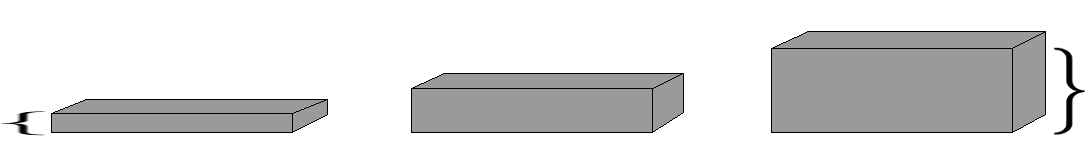
\includegraphics[width=\linewidth]{extrabilder_fuer_vortrag/Introduction2.jpg}
		\end{column}
			\hspace{-15px} 
		\begin{column}{0.1\linewidth}
			\vspace{.2px}
			$\approx~2.7 \unit{nm}$
		\end{column}
	\end{columns}
	\note{The calculations I performed were ab-initio calculations and therefore I used the density functional theory with the exchange-correlation function method PBE, which is short for Perdew-Burke-Ernzerhof through FHI-aims.\\}
	\note{HgTe was examined in thin films from approximately 0.5 nm to 2.7 nm, which are 4 to 17 layers of atoms. Surfaces can only be examined in one direction at once. Because otherwise it would went beyond the scope of a bachelor thesis, we chose just direction of observance, namely the (001) direction. \\
	The main goal this thesis pursued was examining the evolution of topological surface states for different slab thicknesses. Therefore I will now explain the theory behind the realization of this examination.}
	\begin{block}<8->{}
		Main goal: Evolution of surface states in different slab thicknesses.
	\end{block}
\end{frame}

%%% Local Variables:
%%% mode: latex
%%% TeX-master: "main_BA2_Vortrag.tex"
%%% End:
	
	\section{Theory}
	\begin{frame}
	blub
\end{frame}
%%% Local Variables:
%%% mode: latex
%%% TeX-master: "main_BA2_Vortrag.tex"
%%% End:
	
	\section{Results}
	\begin{frame}{lattice constant and k-grid study part 1}
	\begin{columns}
		\begin{column}{0.48\linewidth}
			\centering
			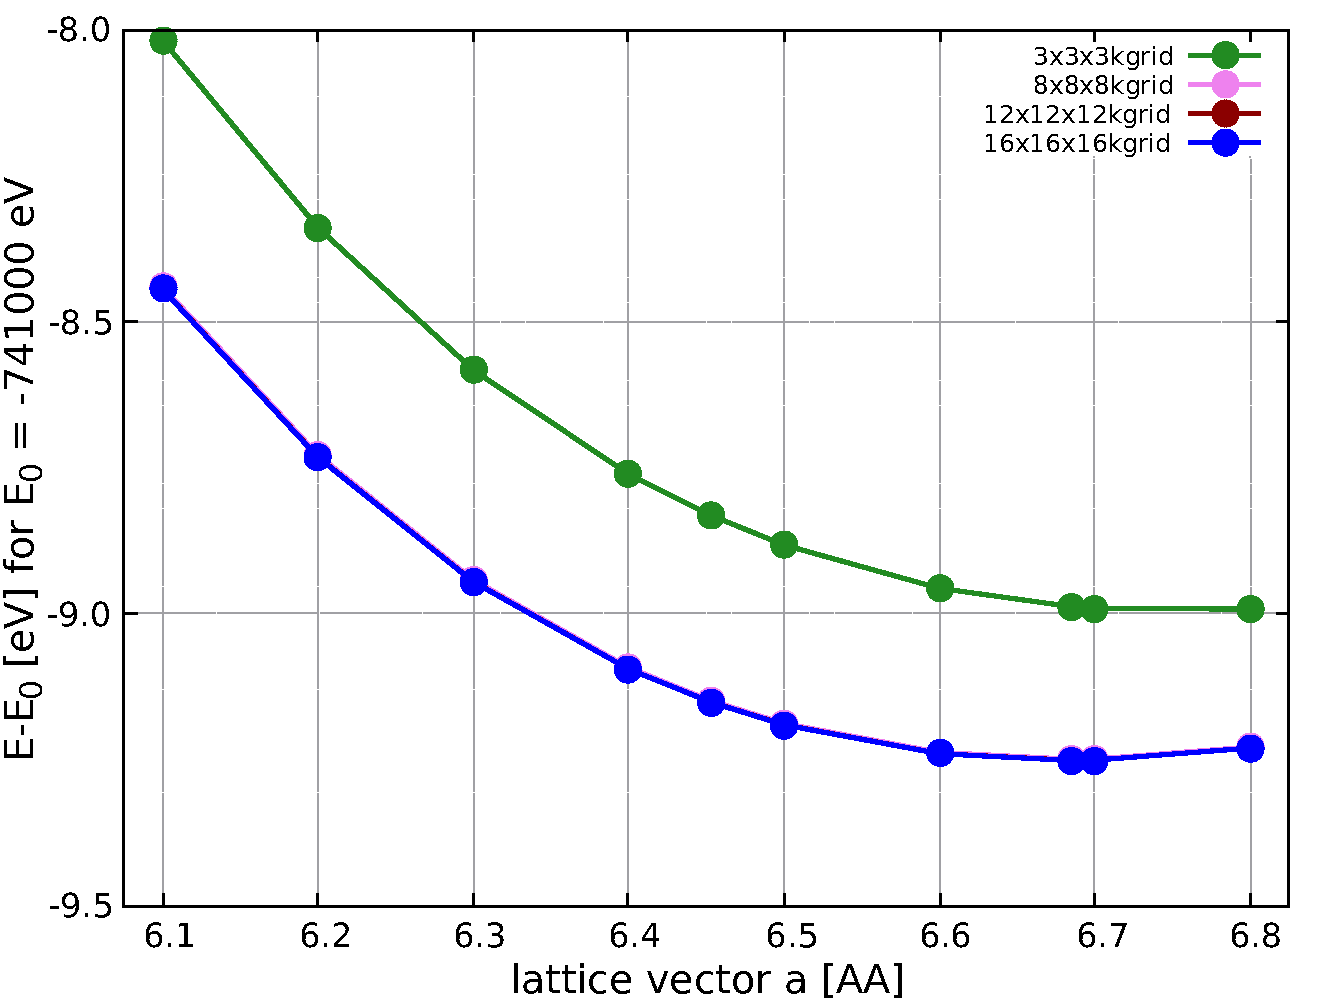
\includegraphics[width=\linewidth]{andere_bilder/plot_energies_hgte_bulk_all_kgrid_in_one.pdf}
			\\
			Lattice constant $a$ with respect to the total energy, calculated with 4 different k-grids. 
		\end{column}
		\begin{column}{0.48\linewidth}
			\centering
			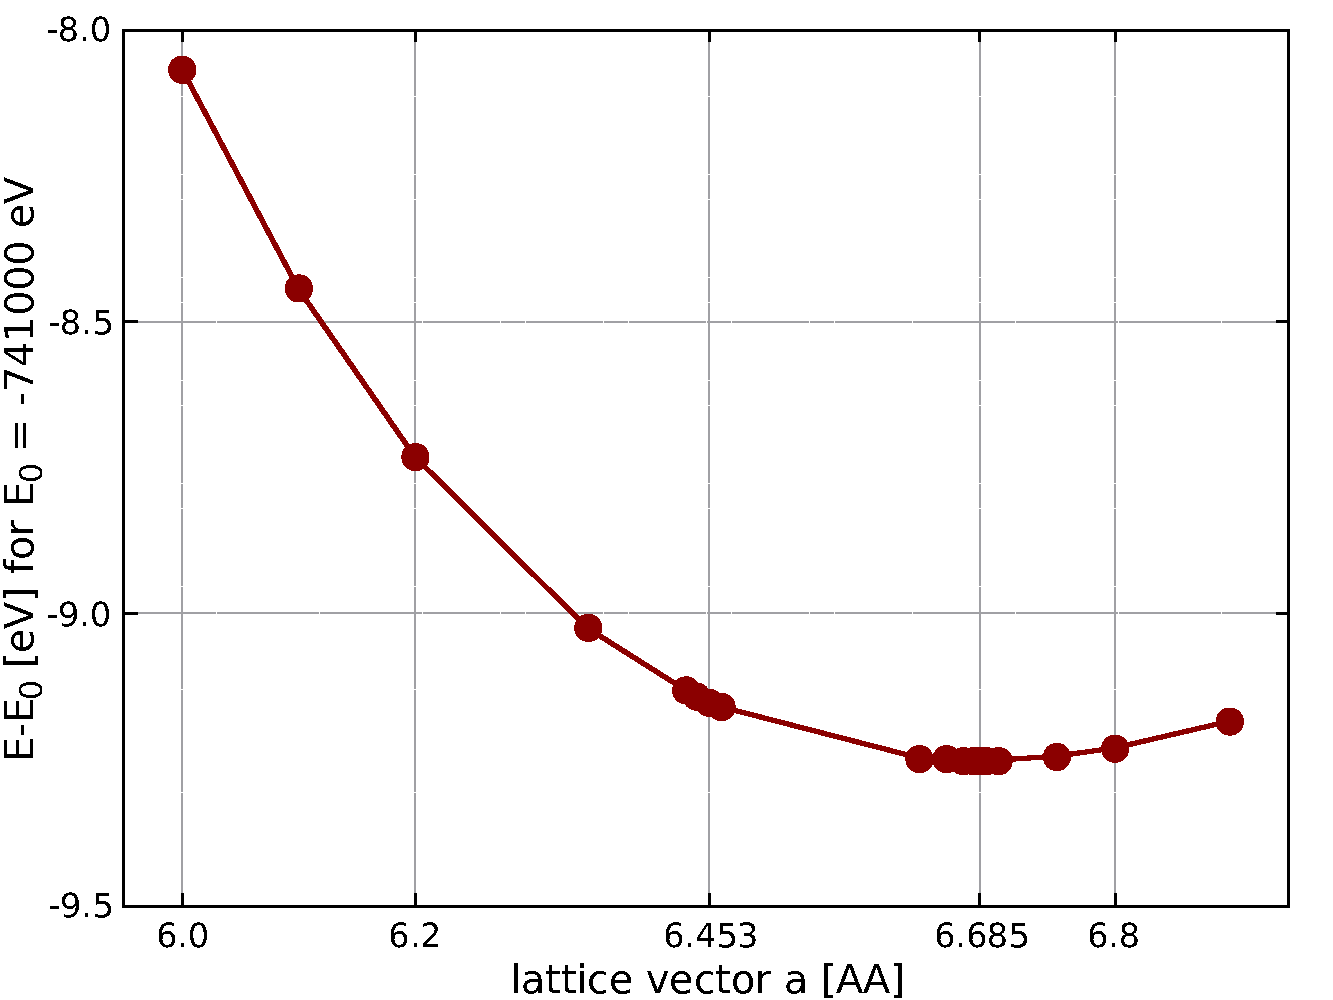
\includegraphics[width=\linewidth]{andere_bilder/lattice_constant_study_spin_none_no_soc.pdf}
			\\
			Lattice constant $a$ with respect to the total energy. The lowest energy was found for 6.685\,$\unit{\AA}$. %\vspace{12.5pt}
		\end{column}
	\end{columns}
	\note{ Let's now turn to the results. First of all I like to mention, that the input data for calculations performed by FHI-aims are the geometry.in and the control.in. The geometry.in contains the coordinates of the lattice vectors and of the atoms. The control.in contains physical settings like the exchange-correlation method, the spin treatment and the relativistic effects. It also contains convergence criteria of the self convergence cycle, the k-grid settings and Informations about all atomic species represented in the geometry.in. \\
	Before starting the calculations for the band structure, it is recommended to do a
	lattice constant study and a k-grid study. So let's have a look at the plot at the left. Here we see the lattice constant with respect to the total energy of the bulk calculated with different k-grids. As we can see the k-grid 3 3 3 gives no good results. The plots for 8 to 16 kgrid overlays, so 8x8x8 seems to be enough to bring physically correct results. In the right picture we see the lattice constant plot for one specific kgrid configuration. The energetically most stable constitution of a crystal structure is given by the lattice constant $a$ with the smallest total system energy, in this case, I found 6.685 Angström for the lowest energy.}
\end{frame}

\begin{frame}{lattice constant and k-grid study part 2}
	\scriptsize{
	Total energy $E [\unit{eV}] - E_0$ (with $E_0$ the energy offset) as a function of k-grid spacing.} \vspace{.1cm}
	\begin{columns}
		\begin{column}{.4\linewidth}
%			\centering
			\scriptsize{
				Bulk: %with $E_0= -741008 \,\unit{eV}$
			}\\ 
			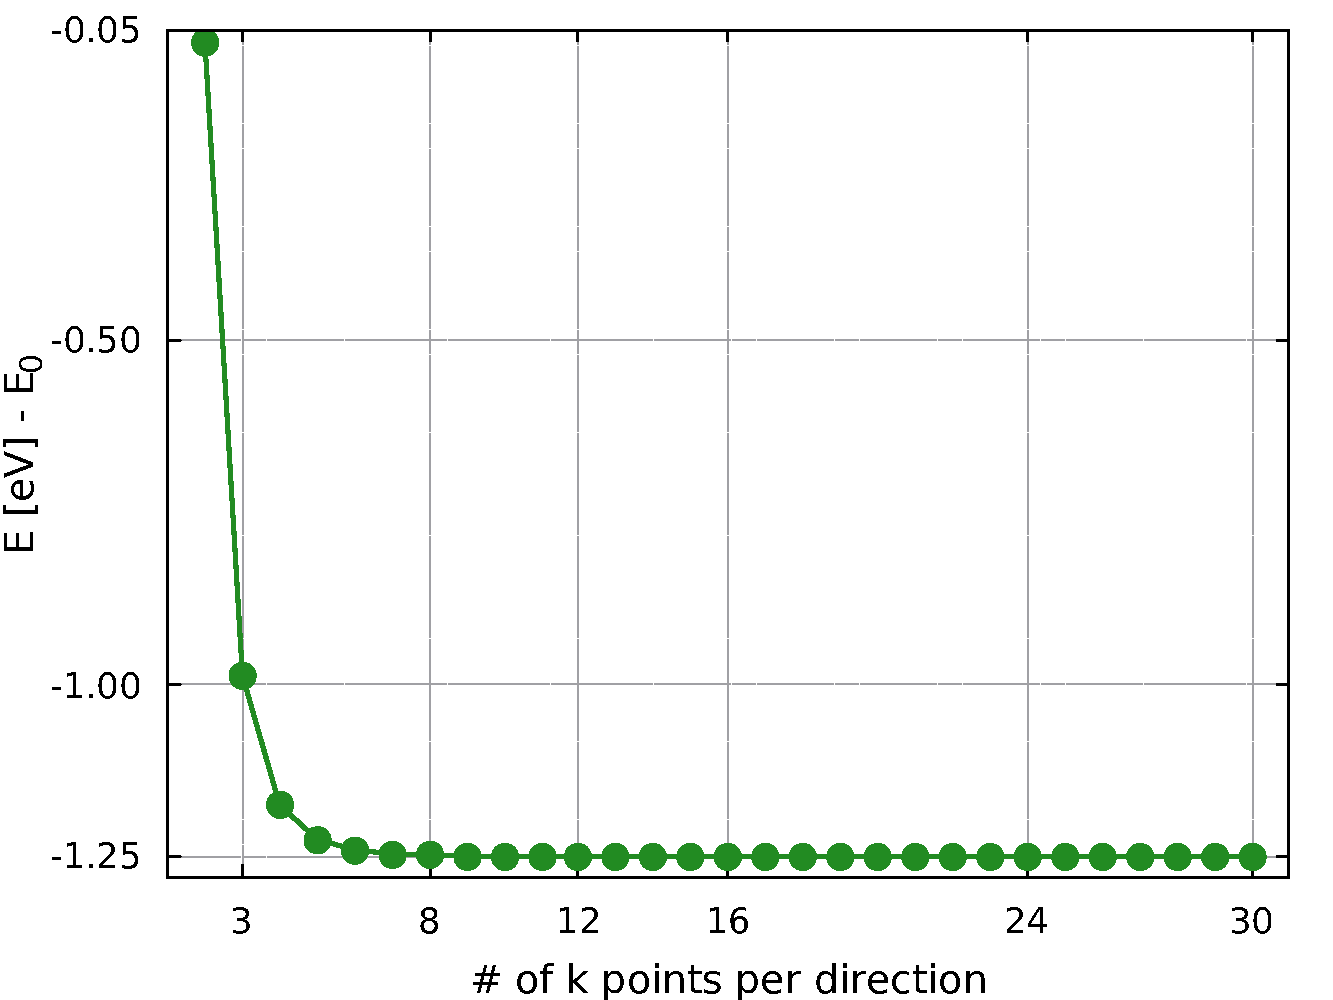
\includegraphics[width=\linewidth]{andere_bilder/kgrid_bulk.pdf}
		\end{column}
		\begin{column}{.4\linewidth}
			\scriptsize{
				Slab with 4 layers: %with $E_0= -1482047 \,\unit{eV}$
			}\\
			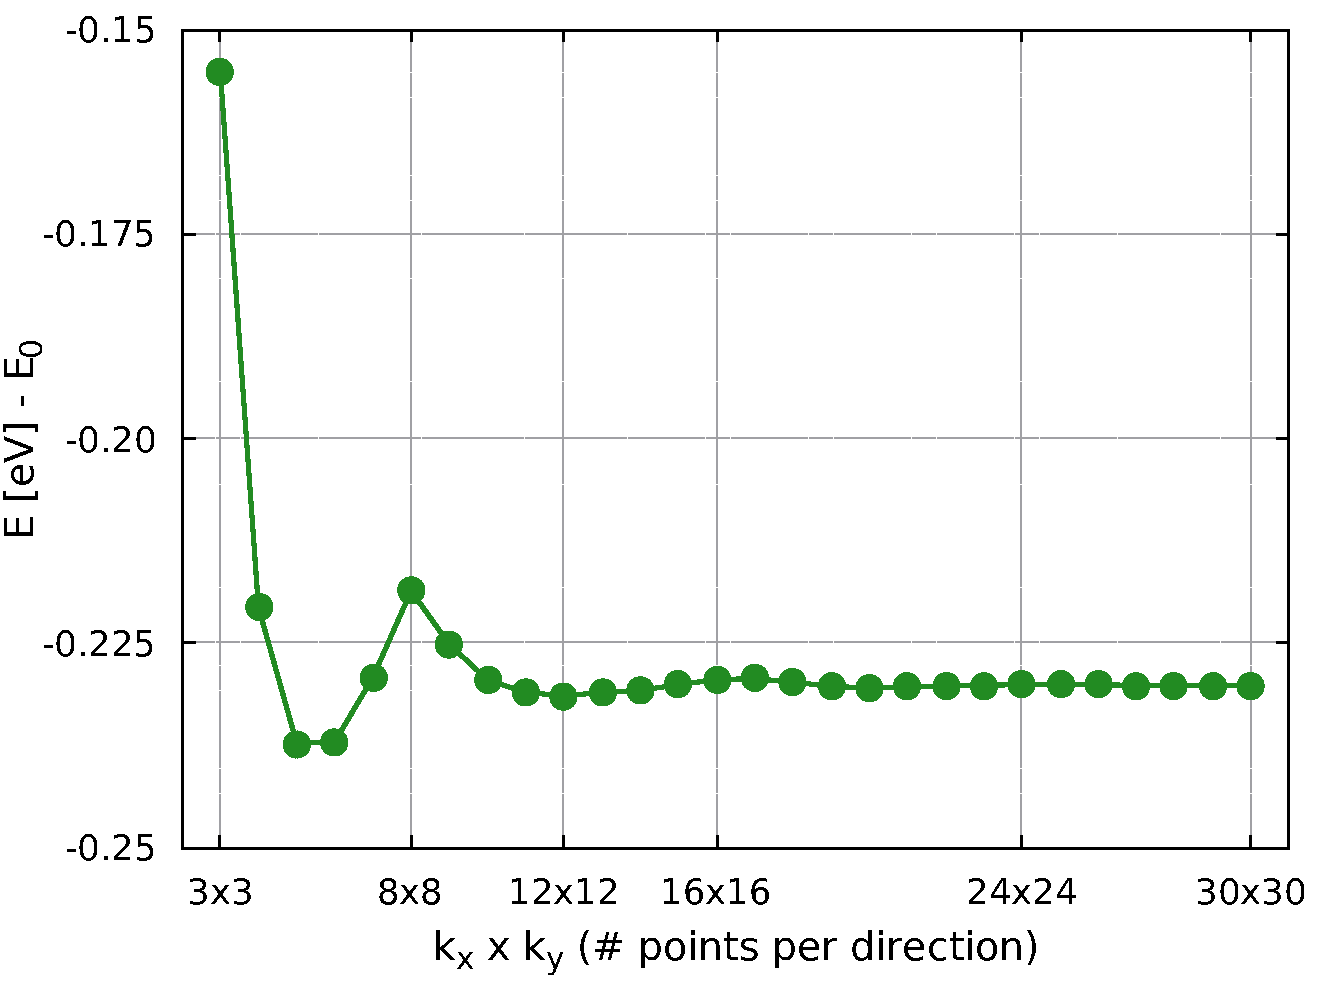
\includegraphics[width=\linewidth]{andere_bilder/kgrid_1x1x4_layers.pdf}
		\end{column}
		\end{columns}
		\begin{columns}
		\begin{column}{.4\linewidth}
			\scriptsize{
				Slab with 8 layers:% with $E_0= -2964065 \,\unit{eV}$
			}\\
			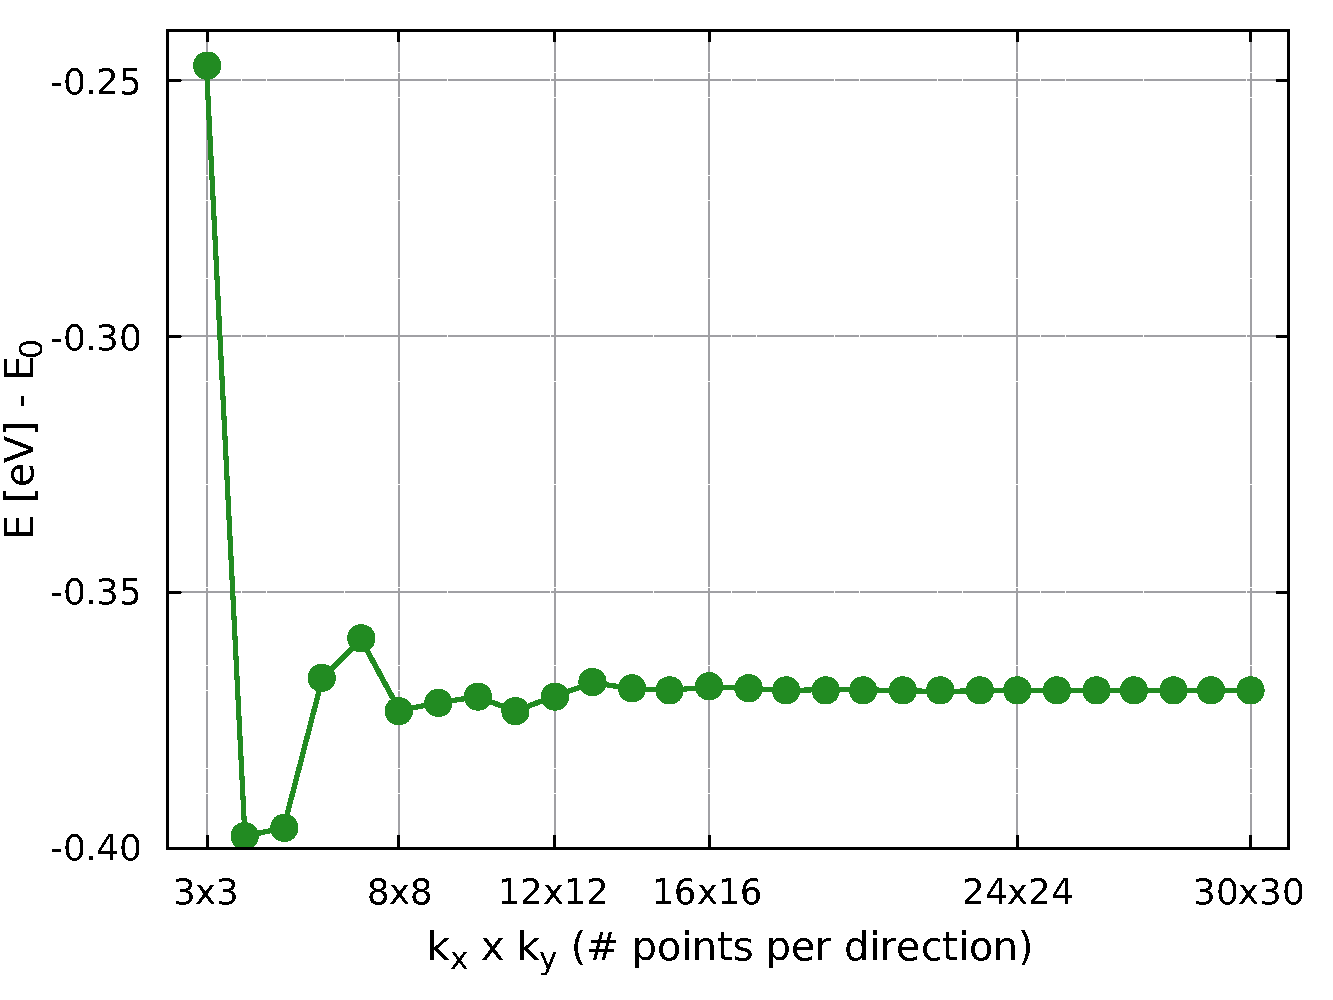
\includegraphics[width=\linewidth]{andere_bilder/kgrid_1x1x8_layers.pdf}
		\end{column}
		\begin{column}{.4\linewidth}
			\scriptsize{
				Slab with 16 layers: %with $E_0= -5928101 \,\unit{eV}$
			} \\
			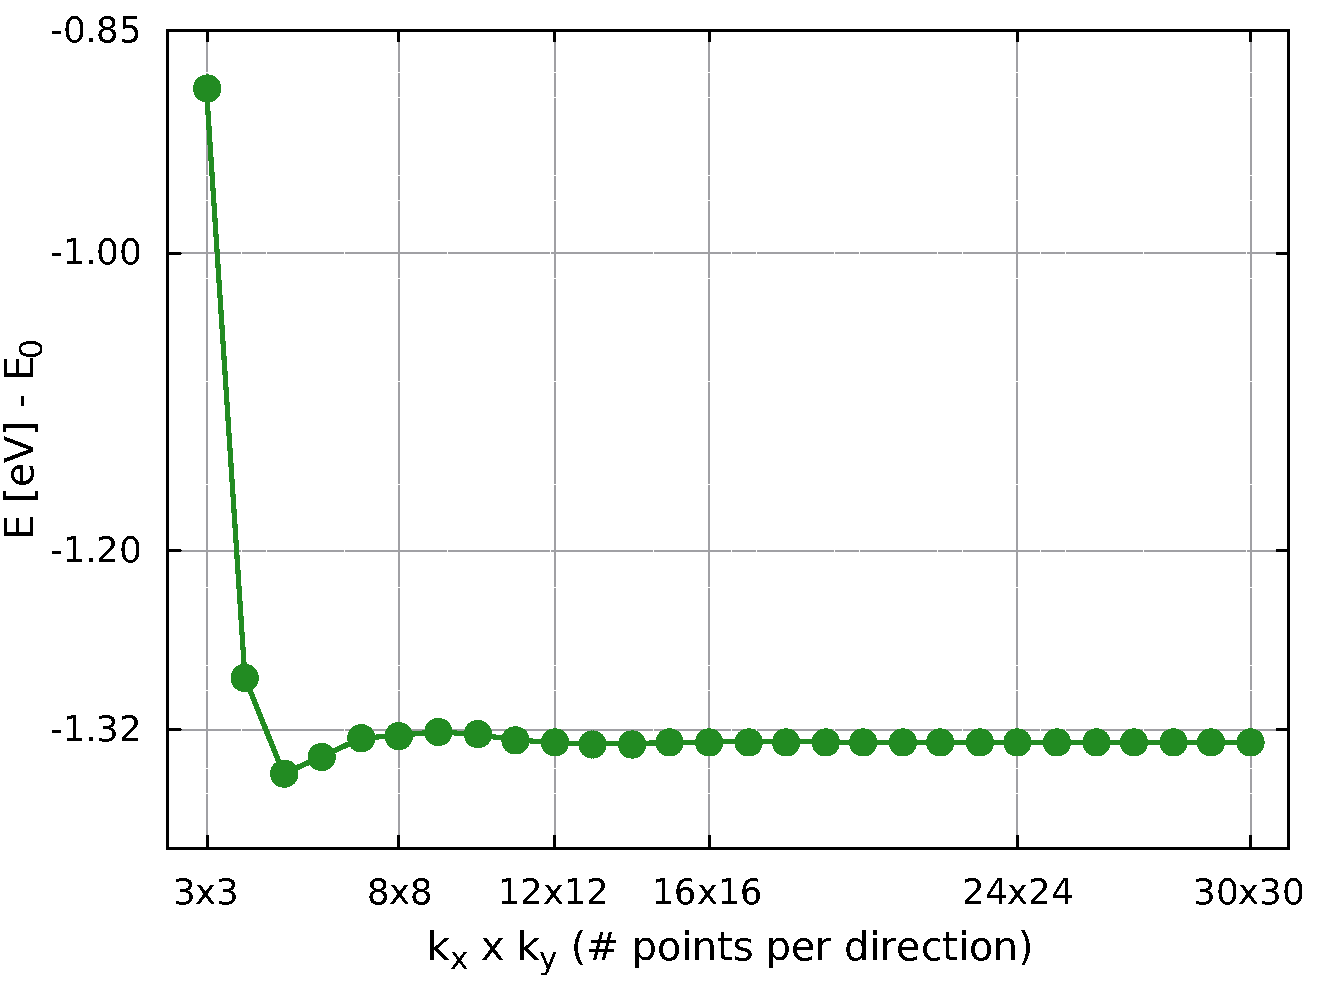
\includegraphics[width=\linewidth]{andere_bilder/kgrid_1x1x16_layers.pdf}
		\end{column}
	\end{columns}
	\note{ This lattice constant then was used for a detailed kgrid study of the bulk and slabs with 4, 8 and 16 layers. Note that for the slabs, k z was set to 1 and that E 0 is just a number different for every plot which was chosen for smaller numbers in the y axis. Since a higher kgrid recommends more computational effort, the most economic kgrid directly after the it has converged to a certain energy. That number was nearly the same for the bulk and the all slabs, namely 12. The oscillation in the plots for the slabs comes from the translation symmetry break in k z direction and therefore it is no wonder that this oscillation becomes smaller for thicker slabs.
	The kgrid used for the following calculations was 24 since higher kgrid gives smoother bands and the additional computational effort was small.}
\end{frame}

\begin{frame}[fragile]{Projected bulk band structure (PBBS)}
	Making 40 slices in 2D Brillouin zone of the bulk from $k_z=0$ to $k_z=k_{z,\text{max}}$ where $k_{z,\text{max}}=\frac{\pi}{a}$. Input example:
	\vspace{-.3cm}
	\begin{columns} 
		\begin{column}<2->{\linewidth}\scriptsize{
			\begin{verbatim}
			output band 0.5   0.0   0.01175   0.0   0.0   0.01175    80  J     Gamma
			output band 0.0   0.0   0.01175   0.5   0.5   0.01175    80  Gamma K
			output band 0.5   0.5   0.01175   0.5   0.0   0.01175    80  K     J
			\end{verbatim} }
		\end{column}
	\end{columns}
	\begin{columns}<3->
		\begin{column}{.165\linewidth} \scriptsize{
				$k_z=0$}
		\end{column} \hspace{-.5cm}
		\begin{column}{.33\linewidth}
%		\begin{figure}[c]{\linewidth}
			\centering
			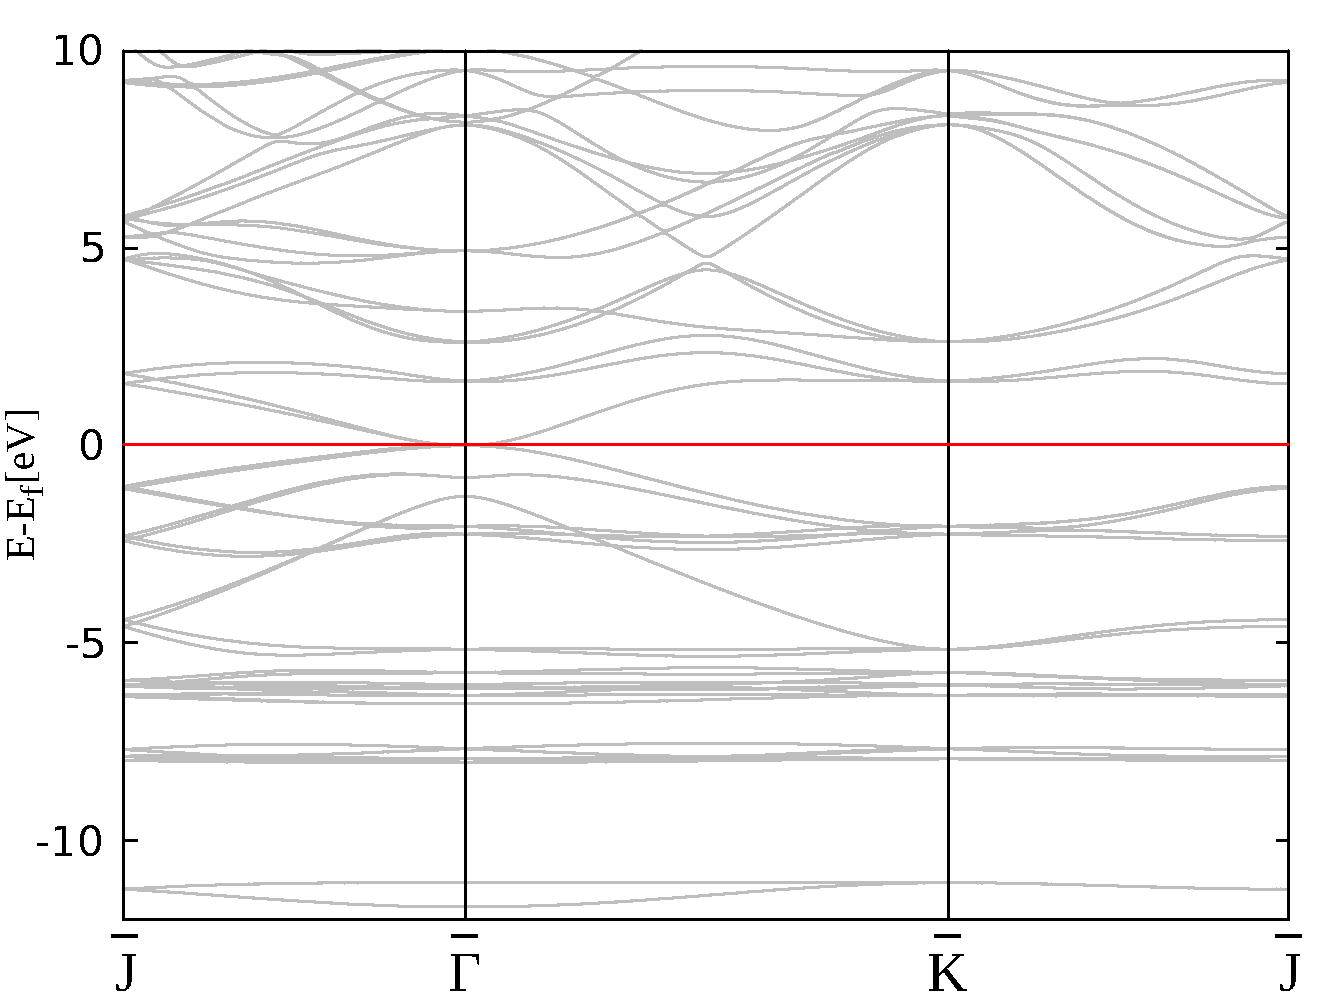
\includegraphics[width=\linewidth]{andere_bilder/0_bulk_-12_10.pdf}
%			\caption{PBBS for $k_z$ is equal to zero.}
%		\end{figure}
		\end{column}
		\begin{column}{.33\linewidth}
%		\begin{figure}[c]{\linewidth}
			\centering
			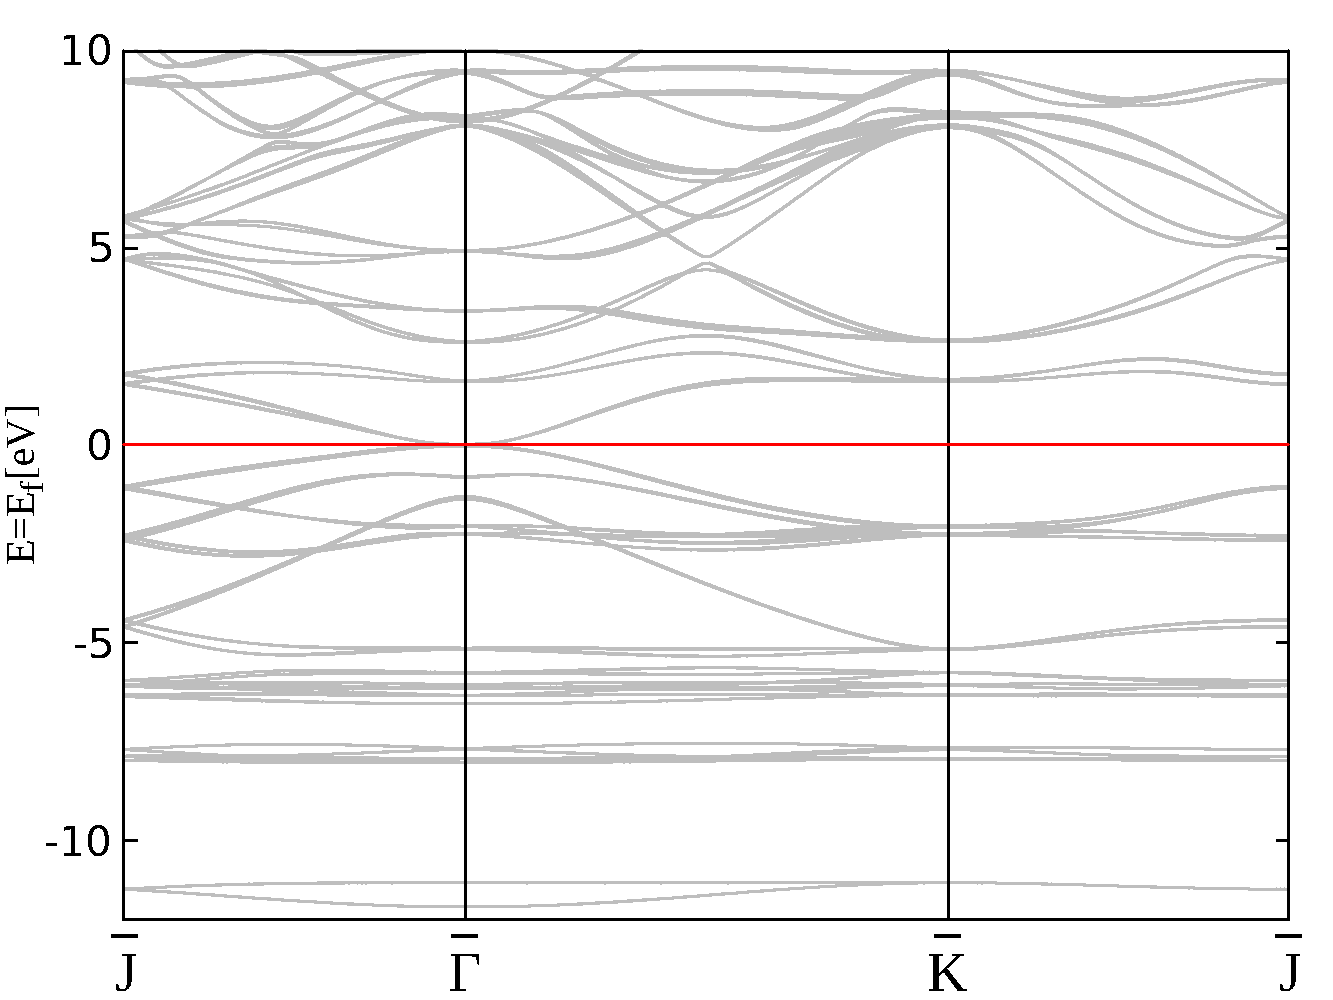
\includegraphics[width=\linewidth]{andere_bilder/4_bulk_-12_10.pdf}
%			\caption{Ensemble for PBBS for $k_z$ having values from 0 to $1/10\cdot k_{z,\text{max}}$}
%		\end{figure}
		\end{column}
		\begin{column}{.165\linewidth} \scriptsize{
			${k_z=0}$ to ${1/10\cdot k_{z,\text{max}}}$ }
		\end{column}
	\end{columns}
	\begin{columns}
		\begin{column}{.165\linewidth} \scriptsize{
				${k_z=0}$ to ${1/4\cdot k_{z,\text{max}}}$ }
		\end{column} \hspace{-.5cm}
		\begin{column}{.33\linewidth}
%		\begin{figure}[c]{\linewidth}
			\centering
			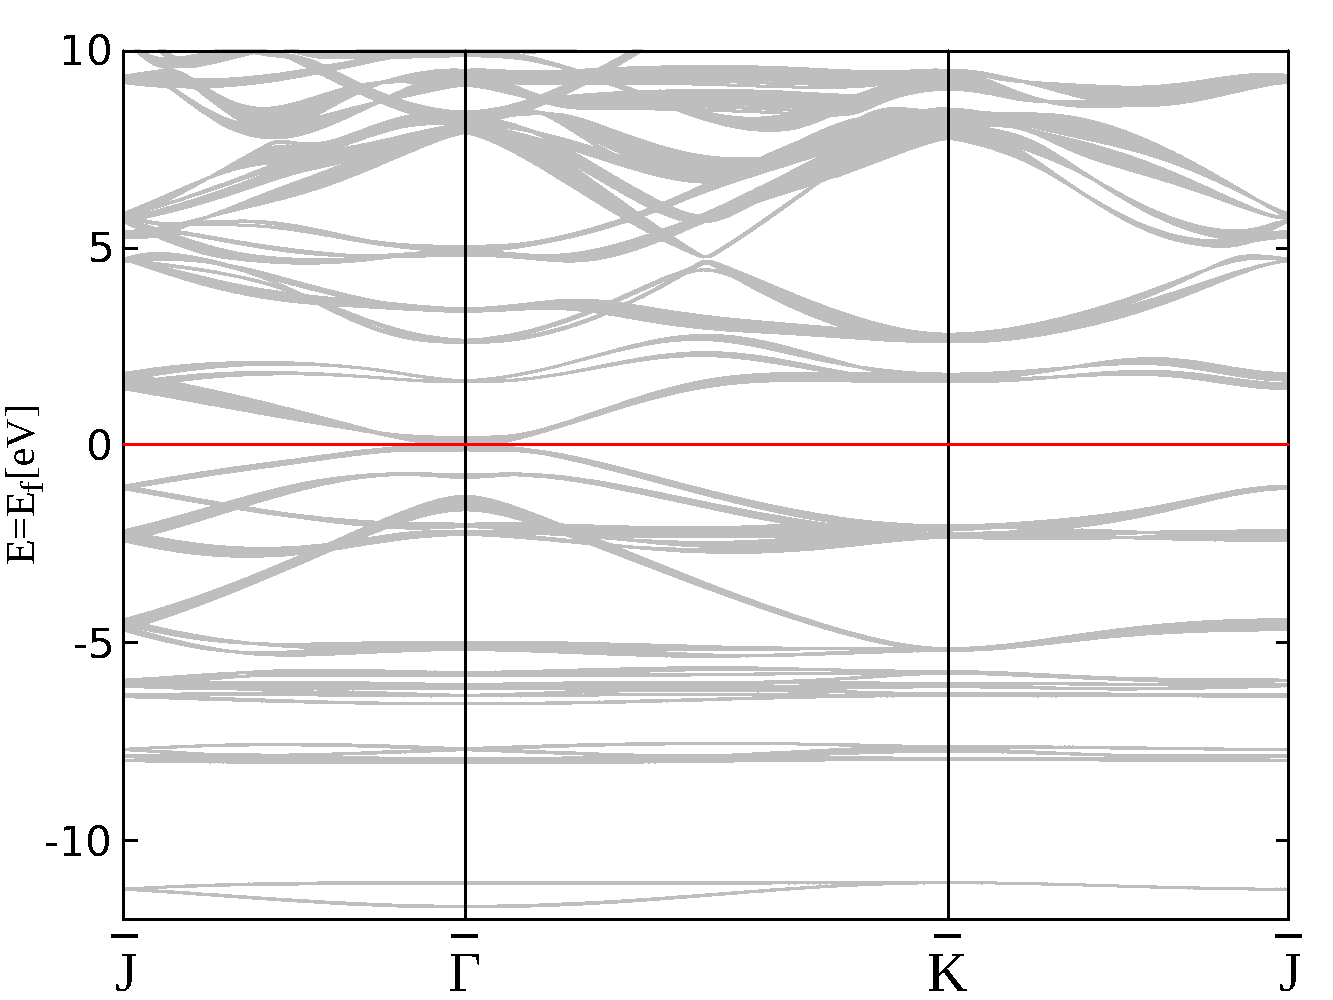
\includegraphics[width=\linewidth]{andere_bilder/10_bulk_-12_10.pdf}
%			\caption{Ensemble for PBBS for $k_z$ having values from 0 to $1/4\cdot k_{z,\text{max}}$} 
%		\end{figure}
		\end{column}
		\begin{column}{.33\linewidth}
%		\begin{figure}[c]{\linewidth}
			\centering 
			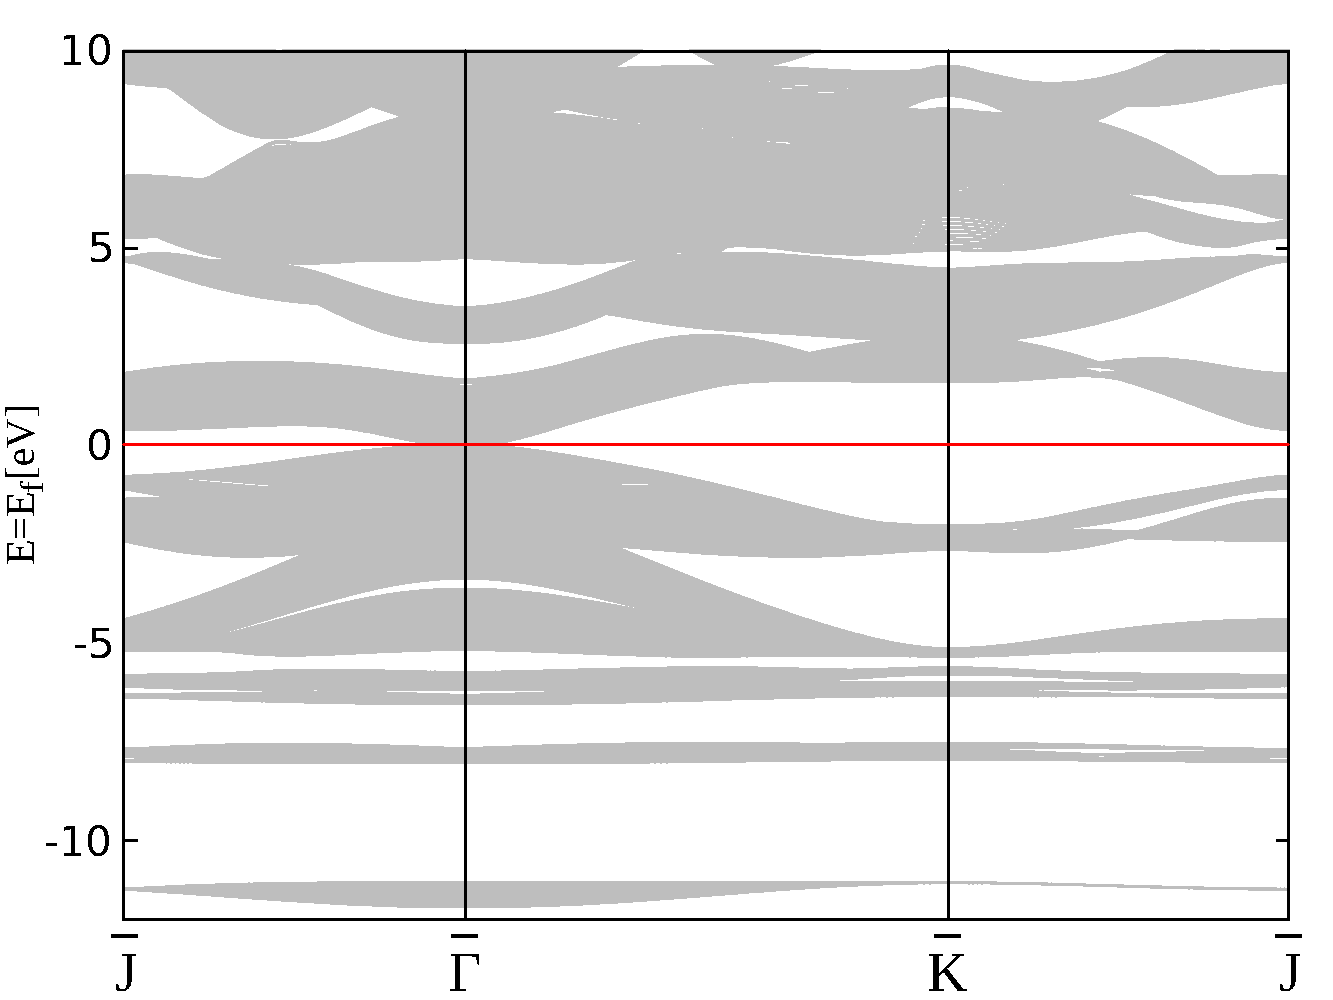
\includegraphics[width=\linewidth]{andere_bilder/bulk_-12_10.pdf}
%			\caption{Whole PBBS for all the values of $k_z$ going from 0 to $k_{z,\text{max}}$} 
%		\end{figure}
		\end{column}
		\begin{column}{.165\linewidth} \scriptsize{
				${k_z=0}$ to $k_{z,\text{max}}$ }
		\end{column}
	\end{columns}	
	\note{ The bulk band structure alone is calculated along the high symmetry points in the 3D Billouin zone. But we want to compare it to the slab band structure with broken symmetry in k z direction. Therefore I used the so-called projected bulk band structure. This means I made a certain amount of slices of the 2D Brillouin zone of the bulk with k z from 0 to k z max which is pi over a. Here you can see an example of the input in the control.in  for kz is one fortieth of k z max. The first three numbers are the coordinates of the high symmetry points where the calculations begin, the fourth to sixth number are the coordinates of the point where the calculations end and 80 are the is the number of points which divides that segment of the path. These pictures show how more and more calculations are added until all results are superposed and the PBBS is complete. The last plot shows the bulk band structure regarded from k z point of view. The grey part is the bulk, the white part symbolizes the gaps. }
\end{frame}


\begin{frame}{PBBS with 4 and 5 layer slabs}
	\begin{columns}
		\begin{column}{.34\linewidth}
			\centering
			Te-Hg termination
		\end{column}
		\begin{column}{.34\linewidth}
			\centering
			Te-Te termination
		\end{column}
		\begin{column}{.34\linewidth}
			\centering
			Hg-Hg termination
		\end{column}
	\end{columns}
	\begin{columns}
		\begin{column}{.34\linewidth}
			\centering
			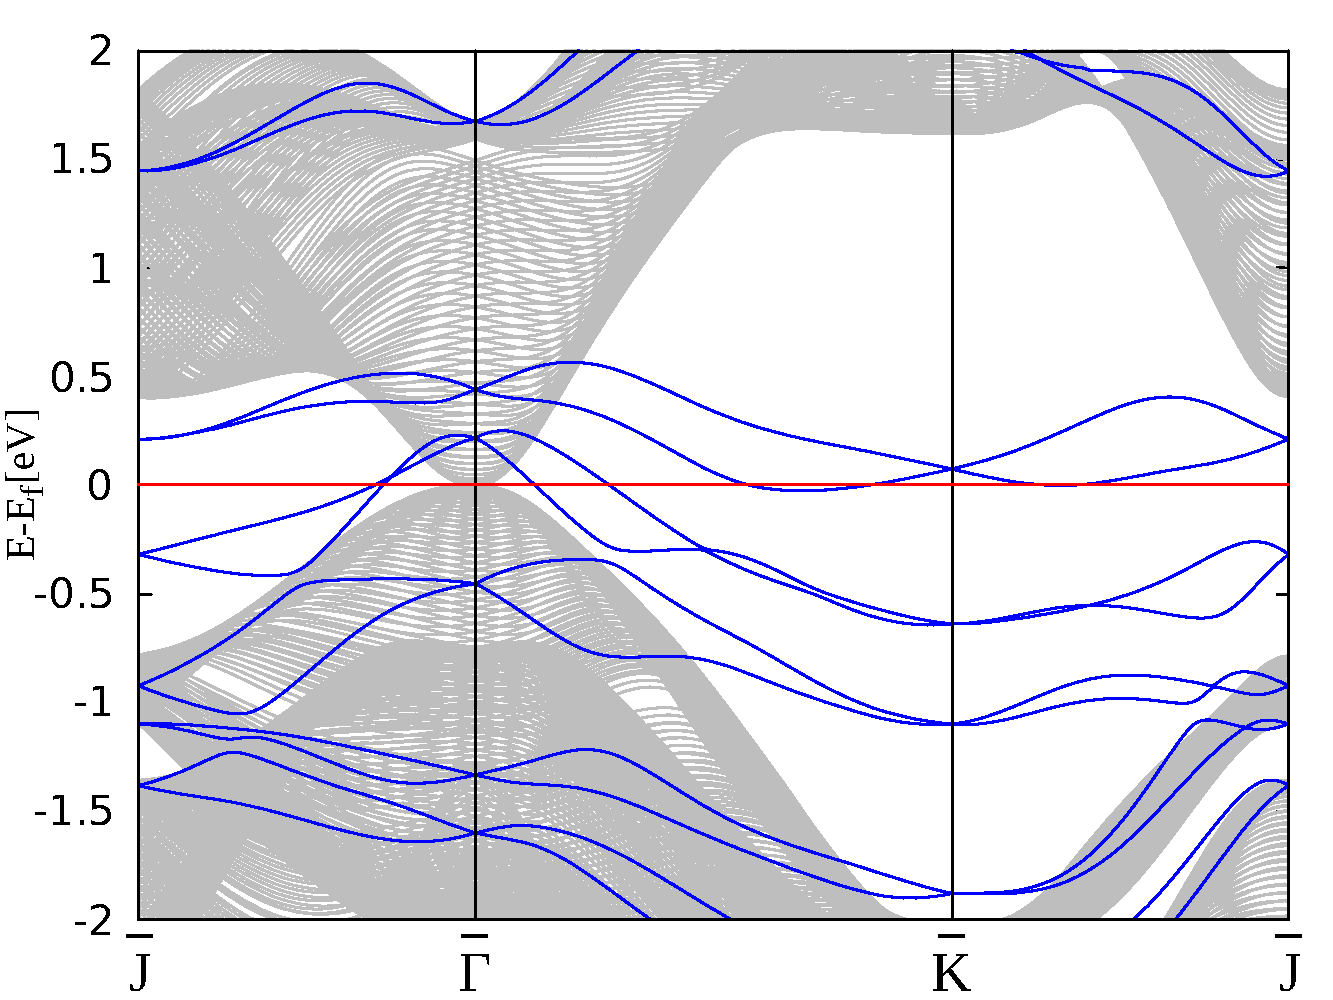
\includegraphics[width=\linewidth]{Te_and_Hg_termination/no_H_bulk+4_layers_no_dos_-2_2.pdf}
%			\caption{4 layers without hydrogens passivating the Te termination}
		\end{column}
		\begin{column}{.34\linewidth}
			\centering
			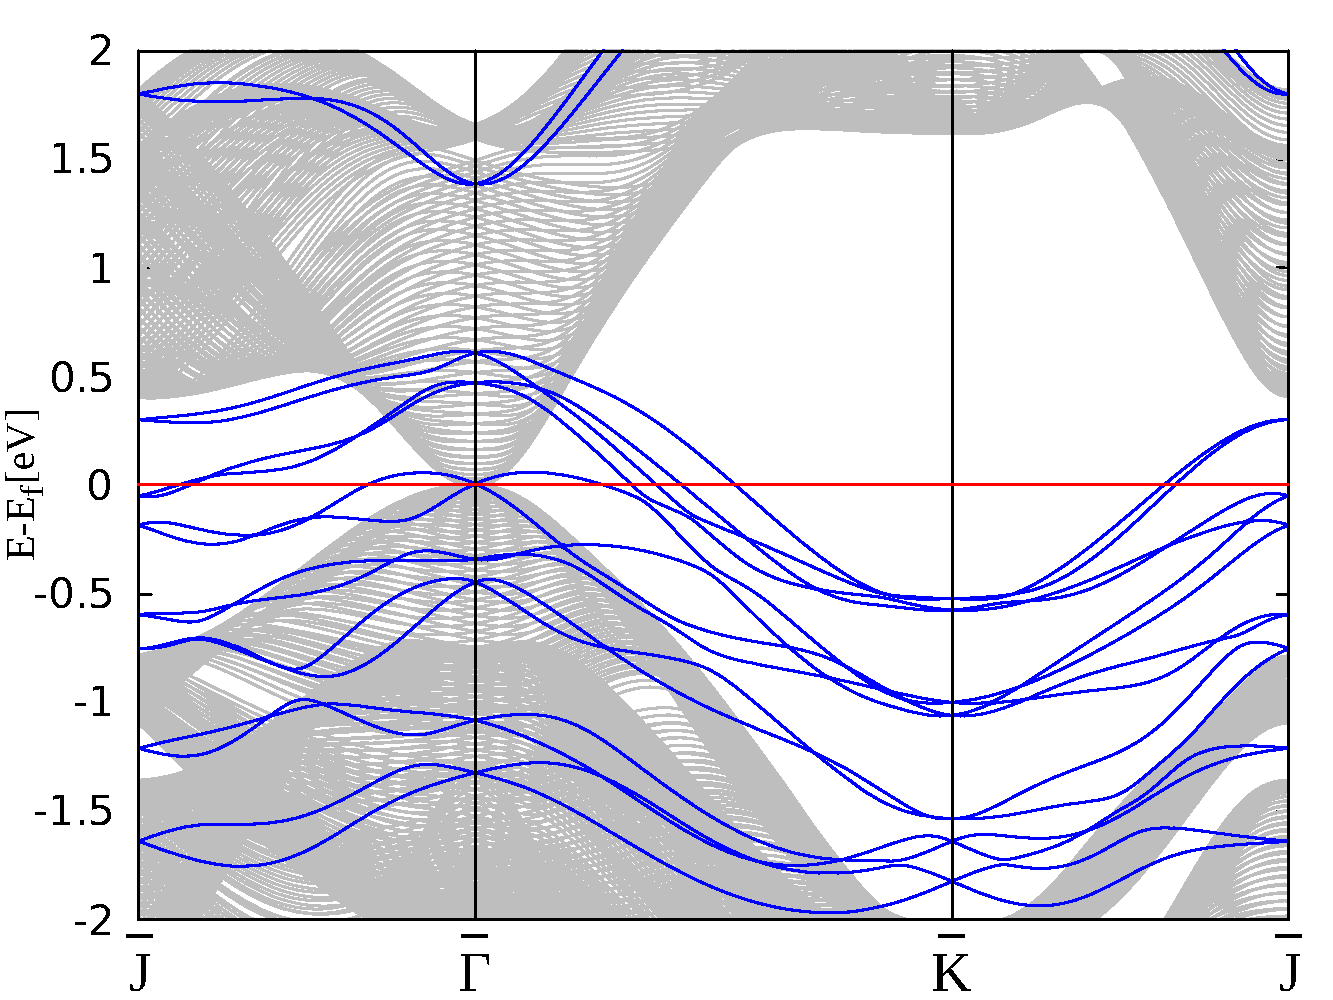
\includegraphics[width=\linewidth]{Te_termination/no_H_bulk+5_layers_no_dos_-2_2.pdf}
%			\caption{5 layers without hydrogens passivating one of the surfaces}
		\end{column}
		\begin{column}{.34\linewidth}
			\centering
			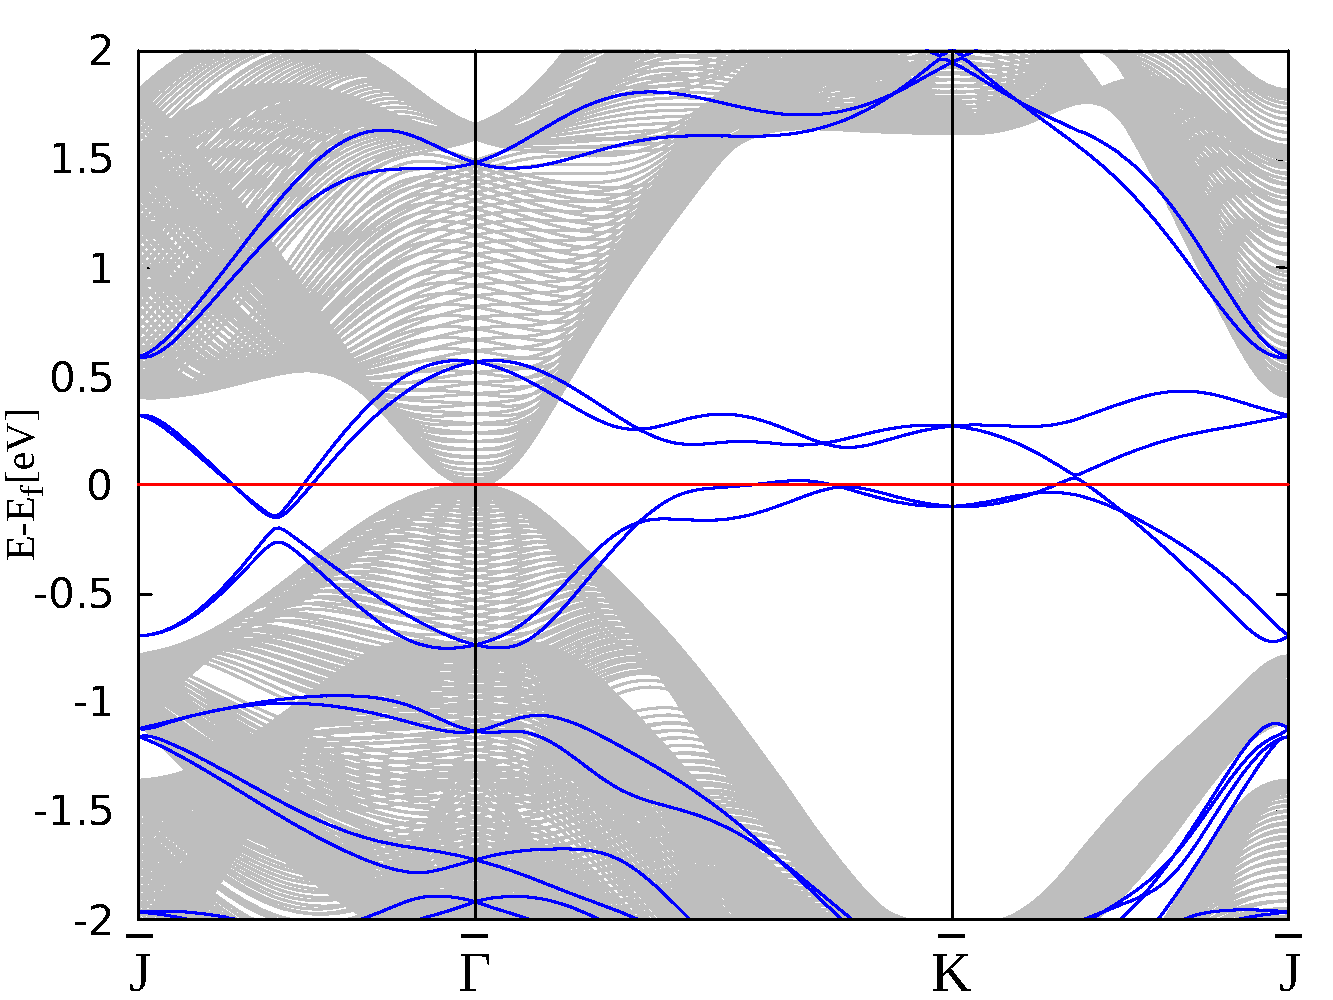
\includegraphics[width=\linewidth]{Hg_termination/no_H_bulk+5_layers_no_dos_-2_2.pdf}
%			\caption{5 layers without hydrogens passivating one of the surfaces}
		\end{column}
	\end{columns}
	\begin{columns}
		\begin{column}{.34\linewidth}
			\centering
			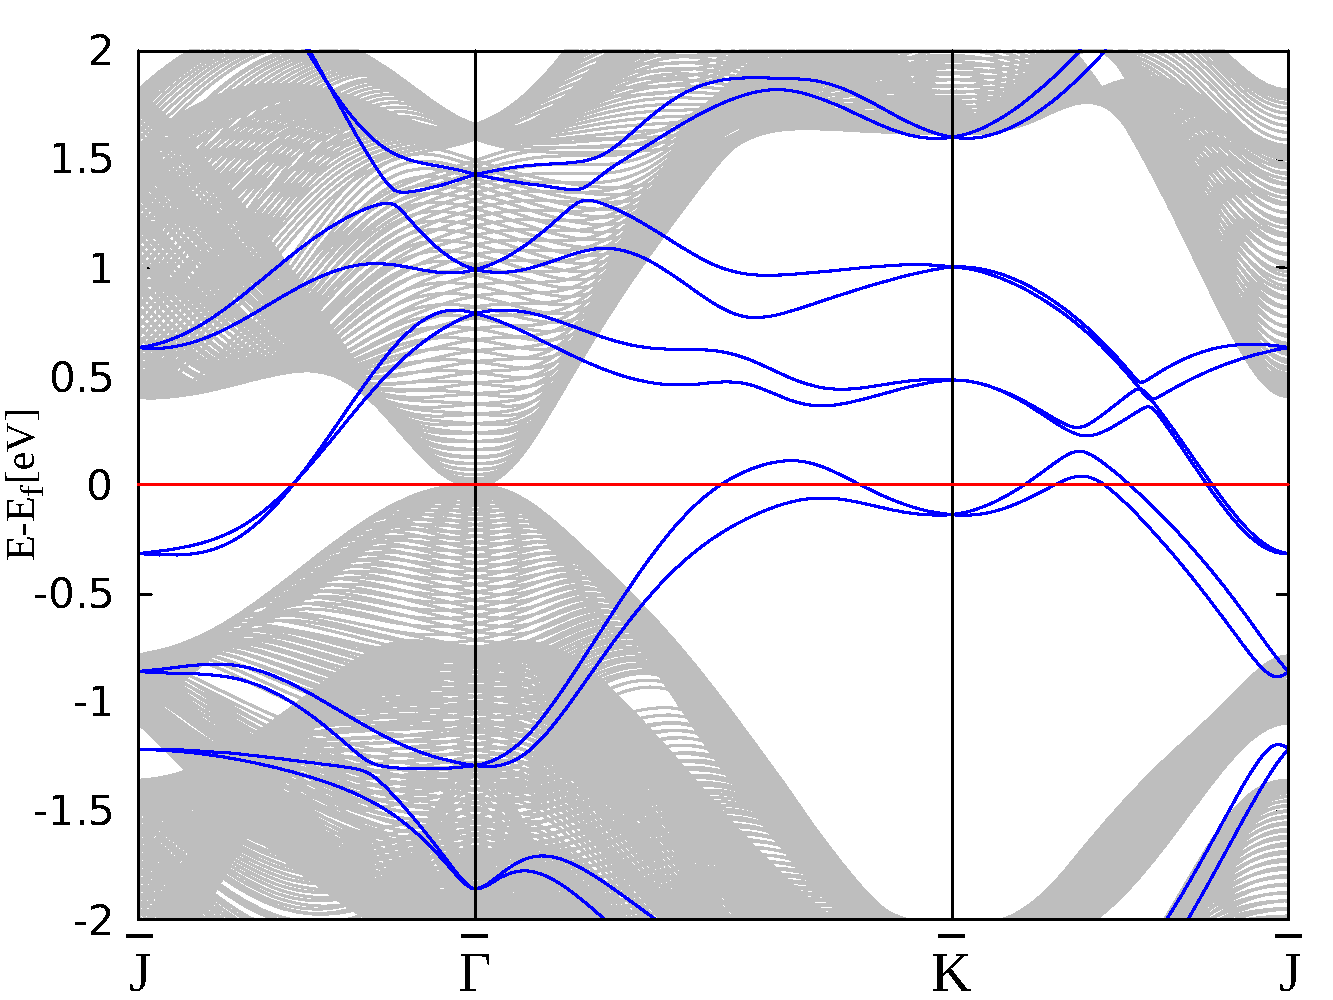
\includegraphics[width=\linewidth]{Te_and_Hg_termination/bulk+4_layers_no_dos_-2_2.pdf}
%			\caption{4 layers with hydrogens on the bottom passivating the Te surface terminations}
		\end{column}
		\begin{column}{.34\linewidth}
			\centering
			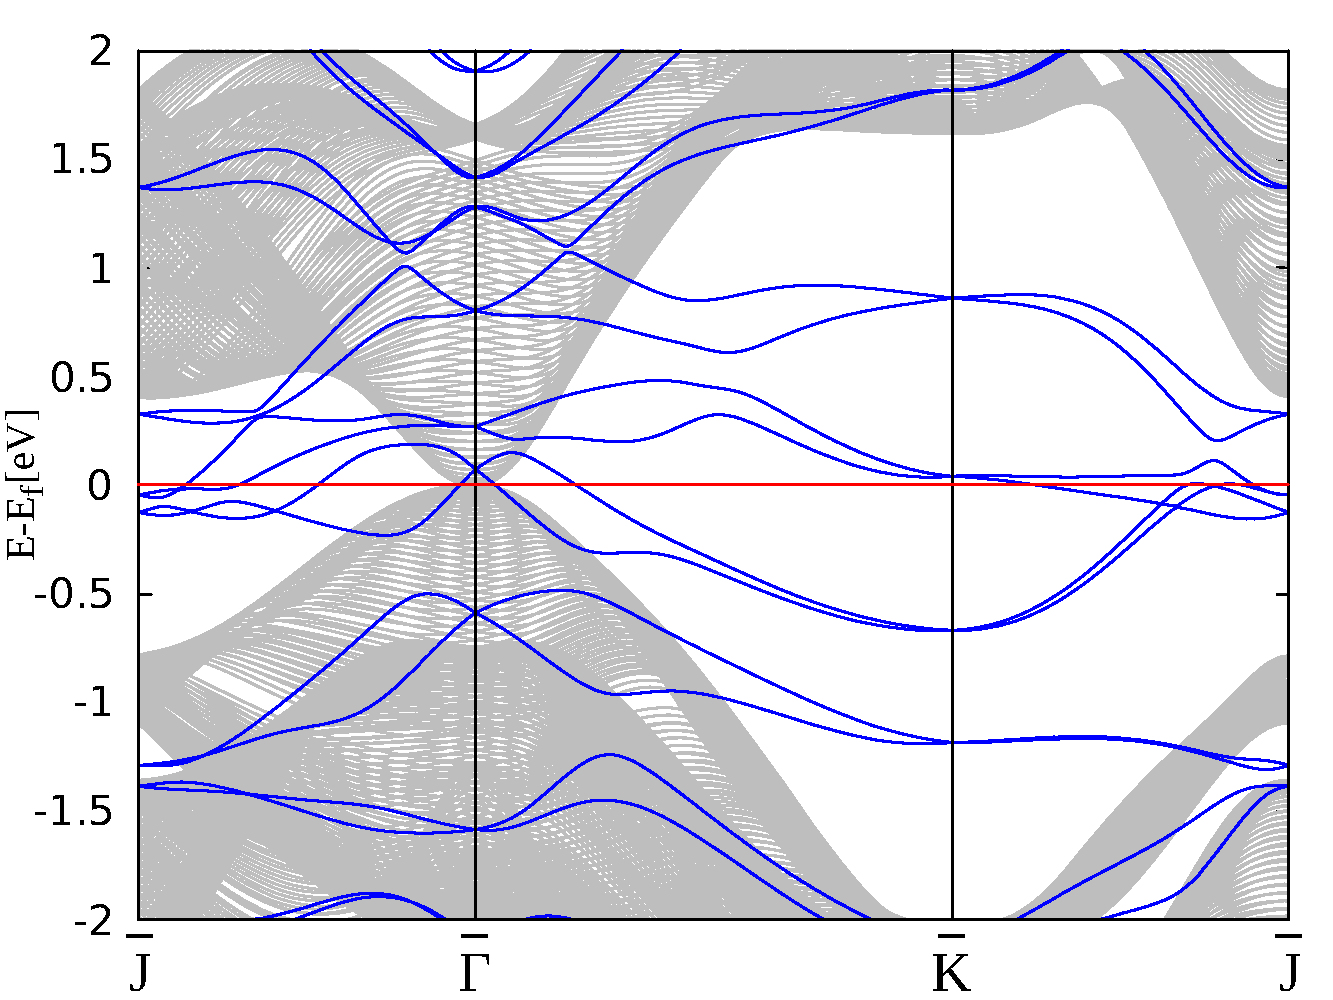
\includegraphics[width=\linewidth]{Te_termination/bulk+5_layers_no_dos_-2_2.pdf}
%			\caption{5 layers with hydrogens on the bottom passivating one of the Te surface terminations}
		\end{column}
		\begin{column}{.34\linewidth}
			\centering
			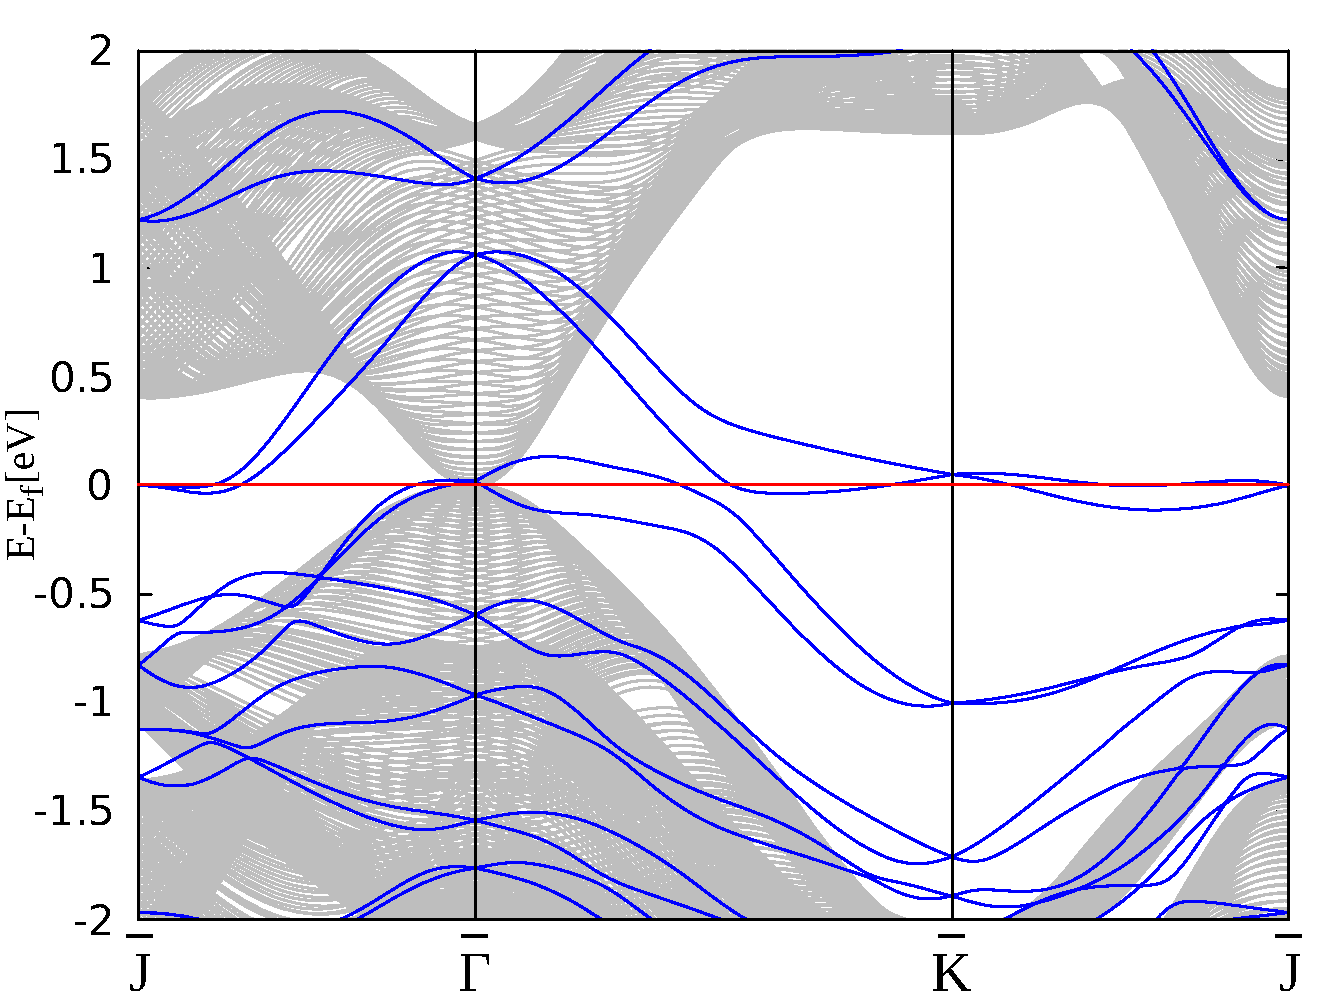
\includegraphics[width=\linewidth]{Hg_termination/bulk+5_layers_no_dos_-2_2.pdf}
%			\caption{5 layers with hydrogens on the bottom passivating one of the Hg surface terminations}
		\end{column}
	\end{columns}
	\vspace{.3cm}
	\footnotesize{
	First row: without hydrogens. \\Second row: with hydrogens passivating one surface.}
	\note{For comparing the PBBS with the slab band structure, I calculated them with the supercell approach and k z set to zero in the band output. The result is then superimposed to the PBBS. As you can see, these (point) are the plots for Te-Hg termination, these (point) for Te-Te and these for Hg-Hg termination, while in this row are all plots for calculations without hydrogens and these plots are all with hydrogens passivating one surface, in case of the Te-Hg termination, the Te surface is passivated. \\
	There are several things one notices while comparing these plots to each other. First of all by looking at them we notice that the slab band structure is very
	sensitive under variation of thickness and terminations: The number of bands rises for thicker slabs. Regarding the slabs with one surface passivated by hydrogens, we can see that the energy bands corresponding to the surface states are shifted away from the Fermi level. In the plots for clean terminations one can observe possible candidates for a Dirac cone (point at gamma point at Fermi level). Slab bands which are completely in the white area are the the surface states, band which are completely in the grey area are bulk bands. Only for 16 and 17 layers we can see bands which are completely in the grey and in the white area. \\
	The surface states which are candidates for topological states must come from valence band an got to the conduction band or vice versa. Additionally one
	can count how many times the dispersion line crosses through the Fermi level. If the
	number of crossings is odd, then this energy band is a topological surface state. When we count those crossings, we only find trivial surface states, which brings us to the conclusion.}
\end{frame}

\begin{frame}{PBBS with 8 and 9 layer slabs}
	\begin{columns}
		\begin{column}{.34\linewidth}
			\centering
			Te-Hg termination
		\end{column}
		\begin{column}{.34\linewidth}
			\centering
			Te-Te termination
		\end{column}
		\begin{column}{.34\linewidth}
			\centering
			Hg-Hg termination
		\end{column}
	\end{columns}
	\begin{columns}
		\begin{column}{.34\linewidth}
			\centering
			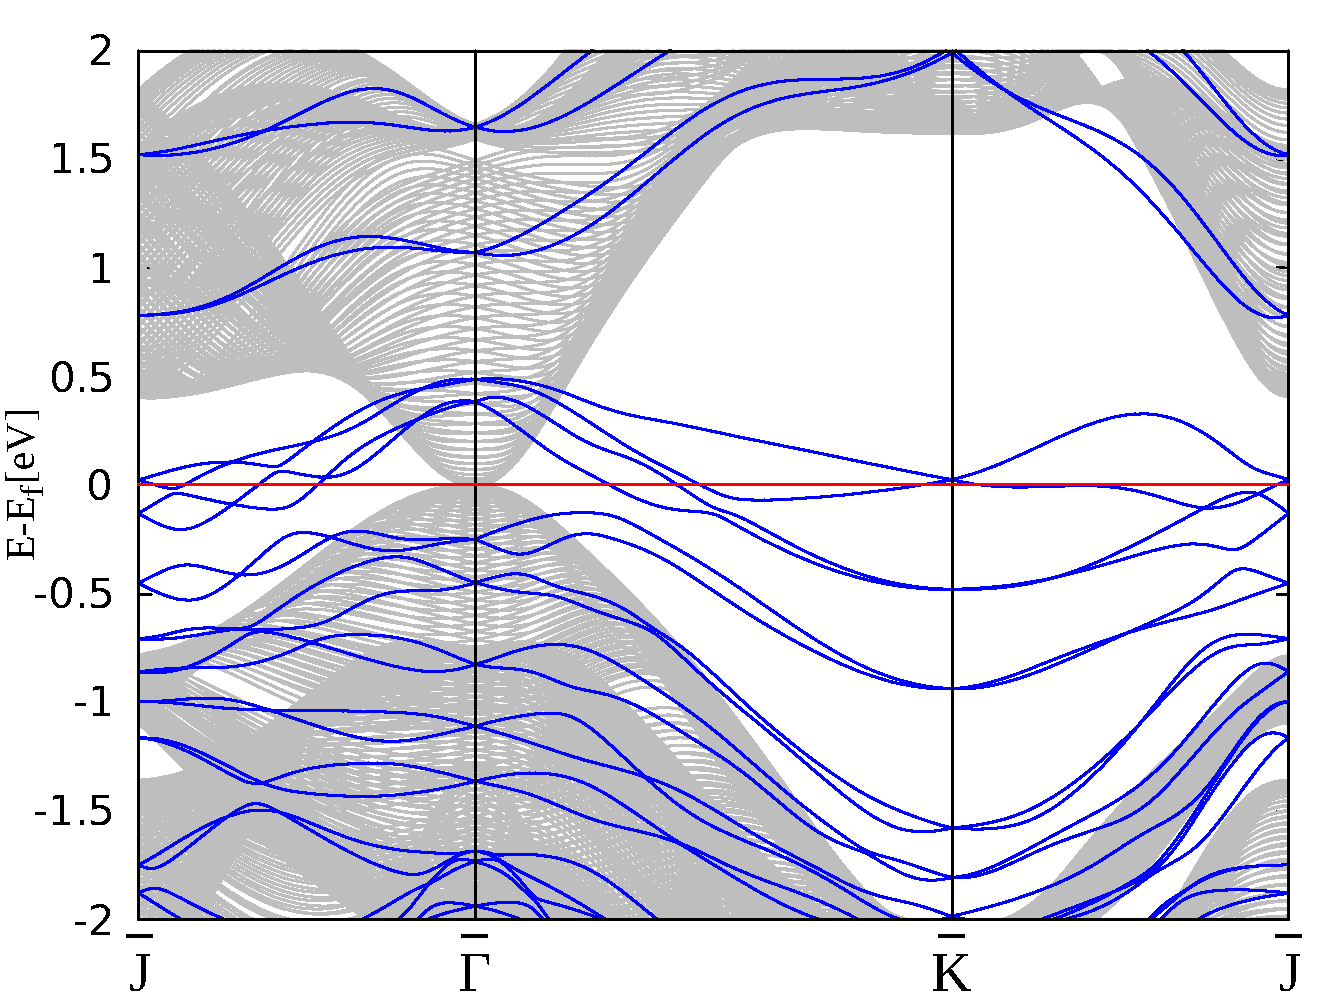
\includegraphics[width=\linewidth]{Te_and_Hg_termination/no_H_bulk+8_layers_no_dos_-2_2.pdf}
%			\caption{8 layers without hydrogens passivating the Te termination}
		\end{column}
		\begin{column}{.34\linewidth}
			\centering
			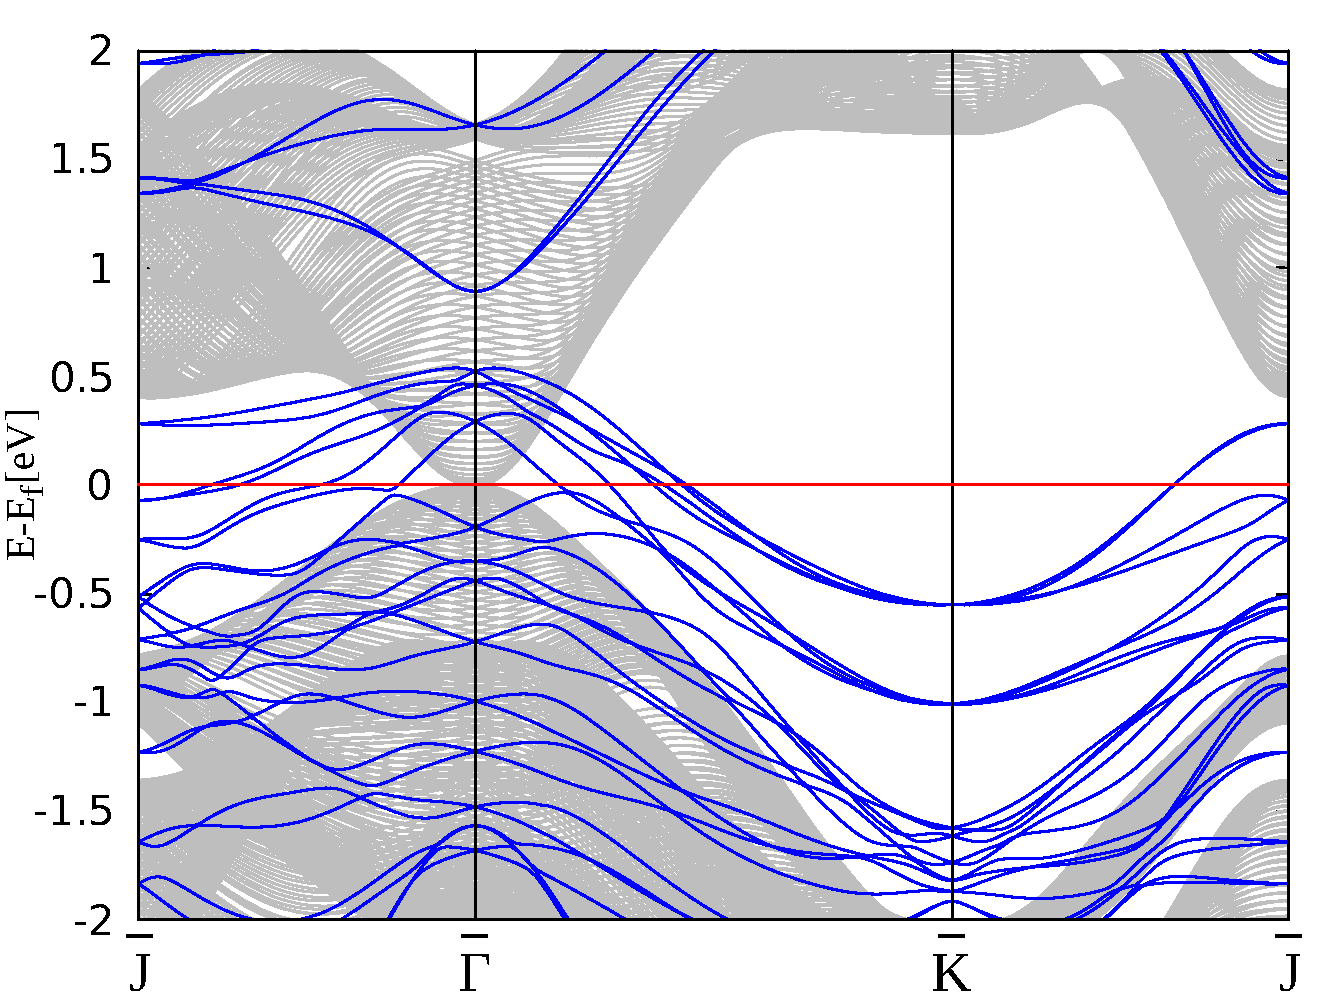
\includegraphics[width=\linewidth]{Te_termination/no_H_bulk+9_layers_no_dos_-2_2.pdf}
%			\caption{9 layers without hydrogens passivating one of the surfaces}
		\end{column}
		\begin{column}{.34\linewidth}
			\centering
			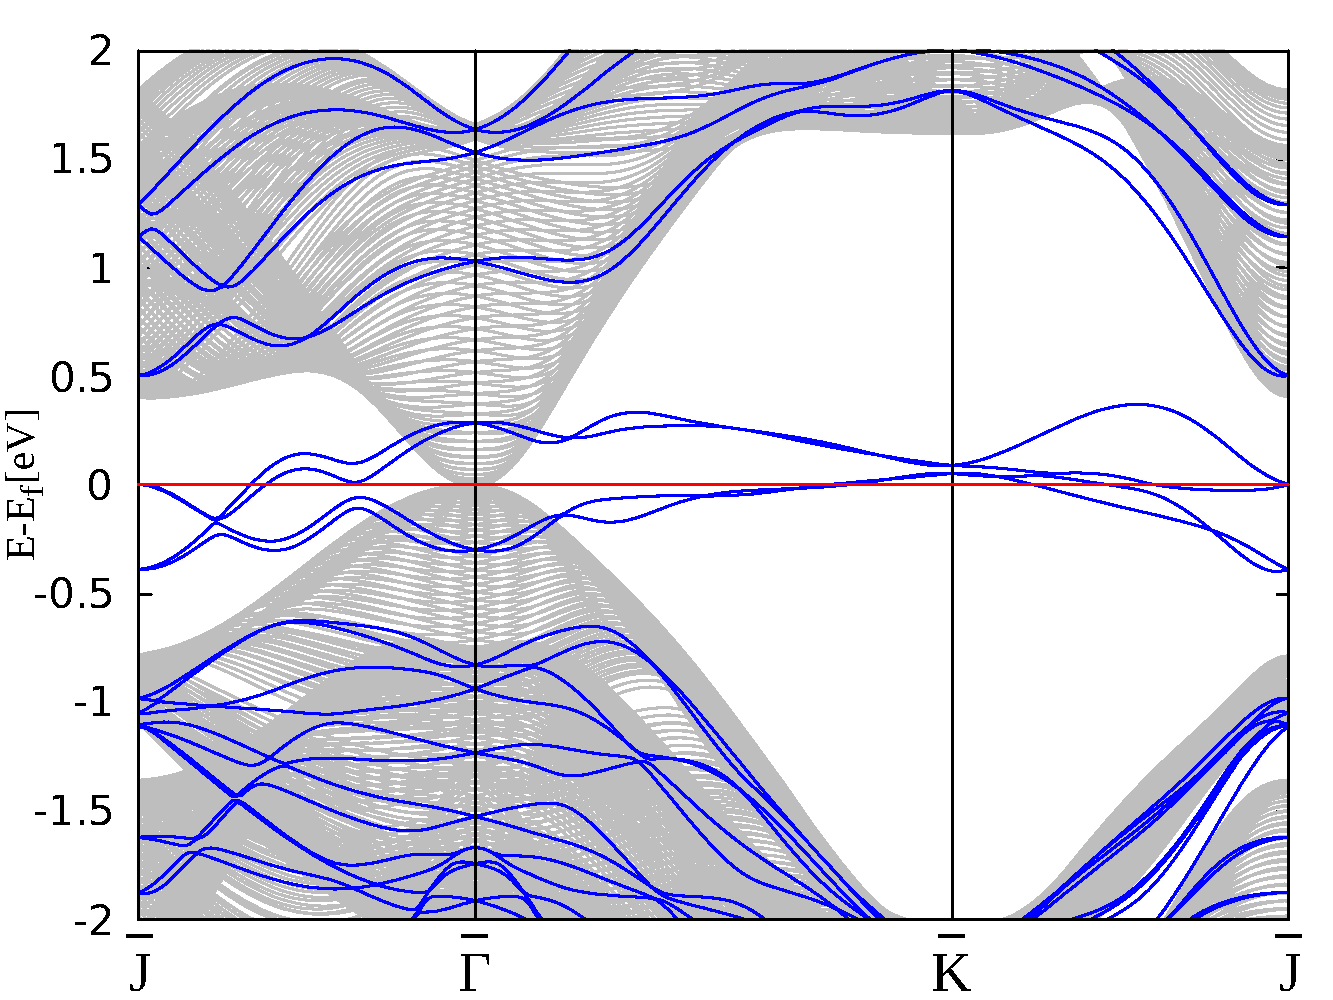
\includegraphics[width=\linewidth]{Hg_termination/no_H_bulk+9_layers_no_dos_-2_2.pdf}
%			\caption{9 layers without hydrogens passivating one of the surfaces}
		\end{column}
	\end{columns}
	\begin{columns}
		\begin{column}{.34\linewidth}
			\centering
			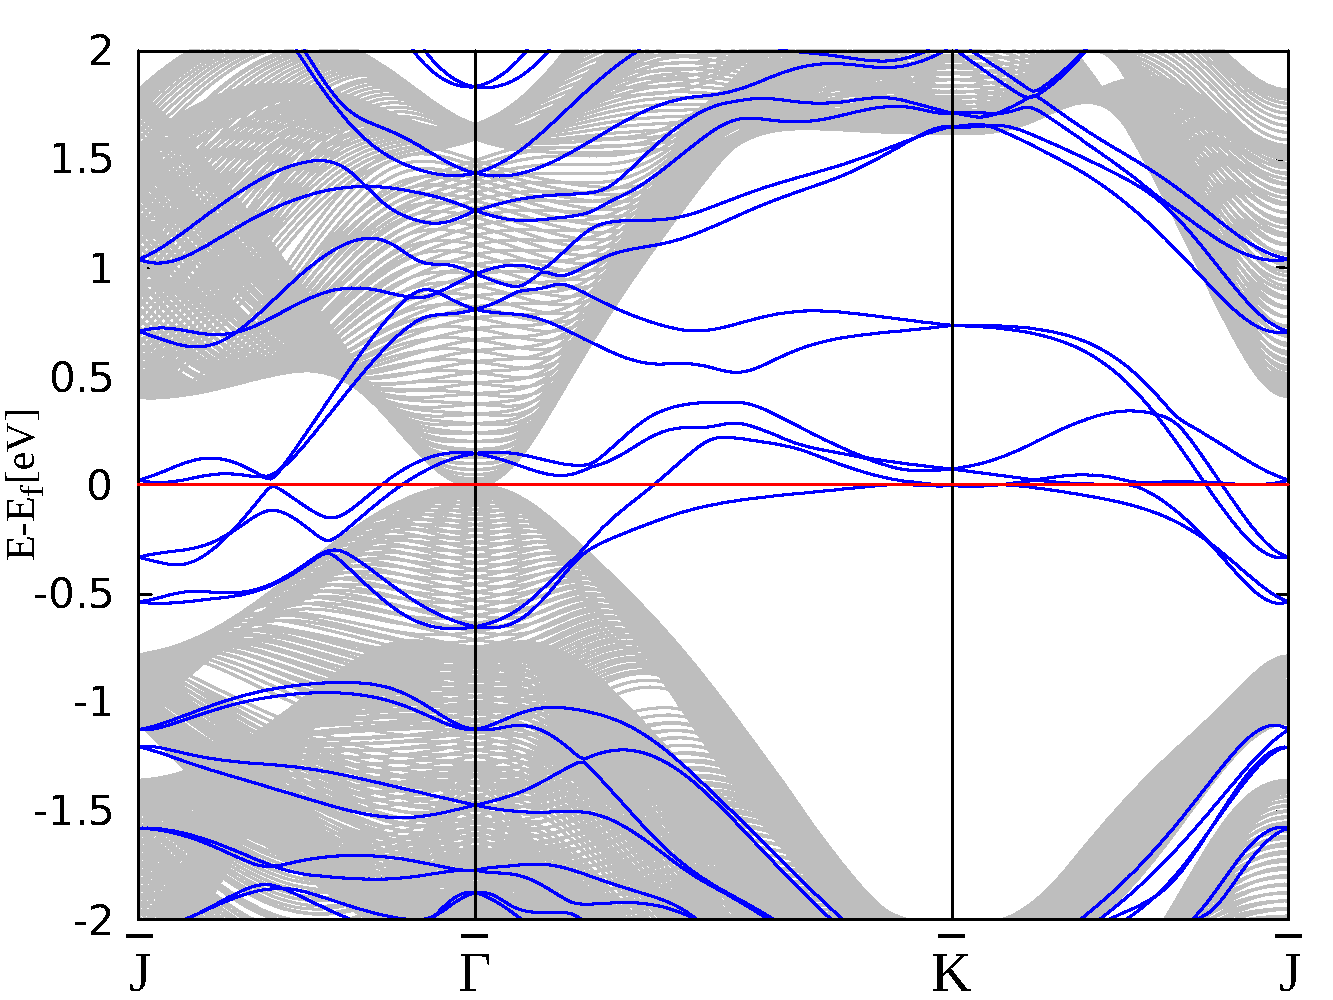
\includegraphics[width=\linewidth]{Te_and_Hg_termination/bulk+8_layers_no_dos_-2_2.pdf}
%			\caption{8 layers with hydrogens on the bottom passivating the Te surface terminations}
		\end{column}
		\begin{column}{.34\linewidth}
			\centering
			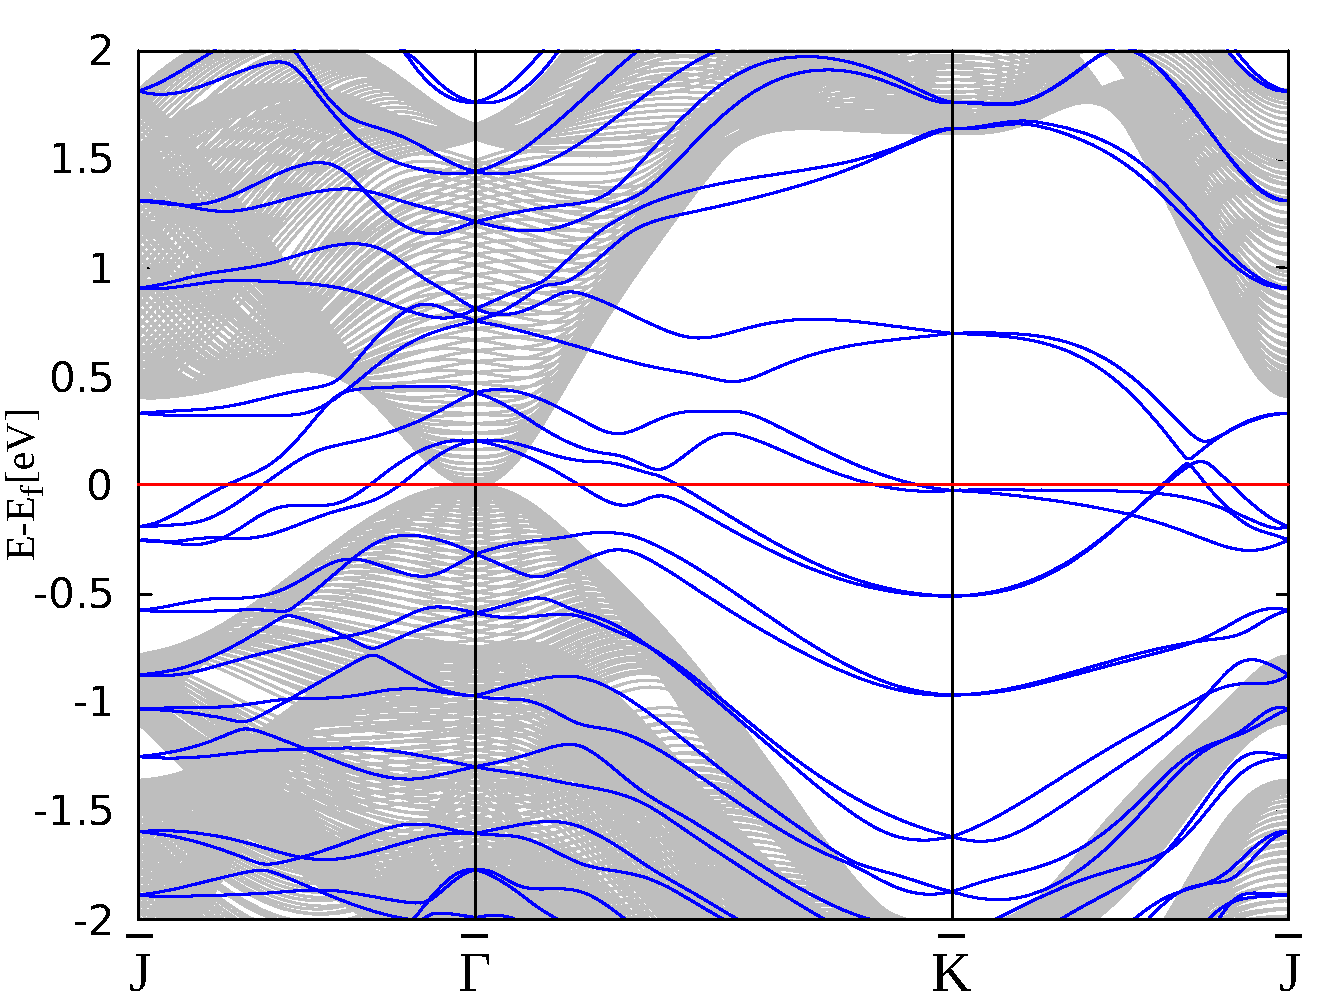
\includegraphics[width=\linewidth]{Te_termination/bulk+9_layers_no_dos_-2_2.pdf}
%			\caption{9 layers with hydrogens on the bottom passivating one of the Te surface terminations}
		\end{column}
		\begin{column}{.34\linewidth}
			\centering
			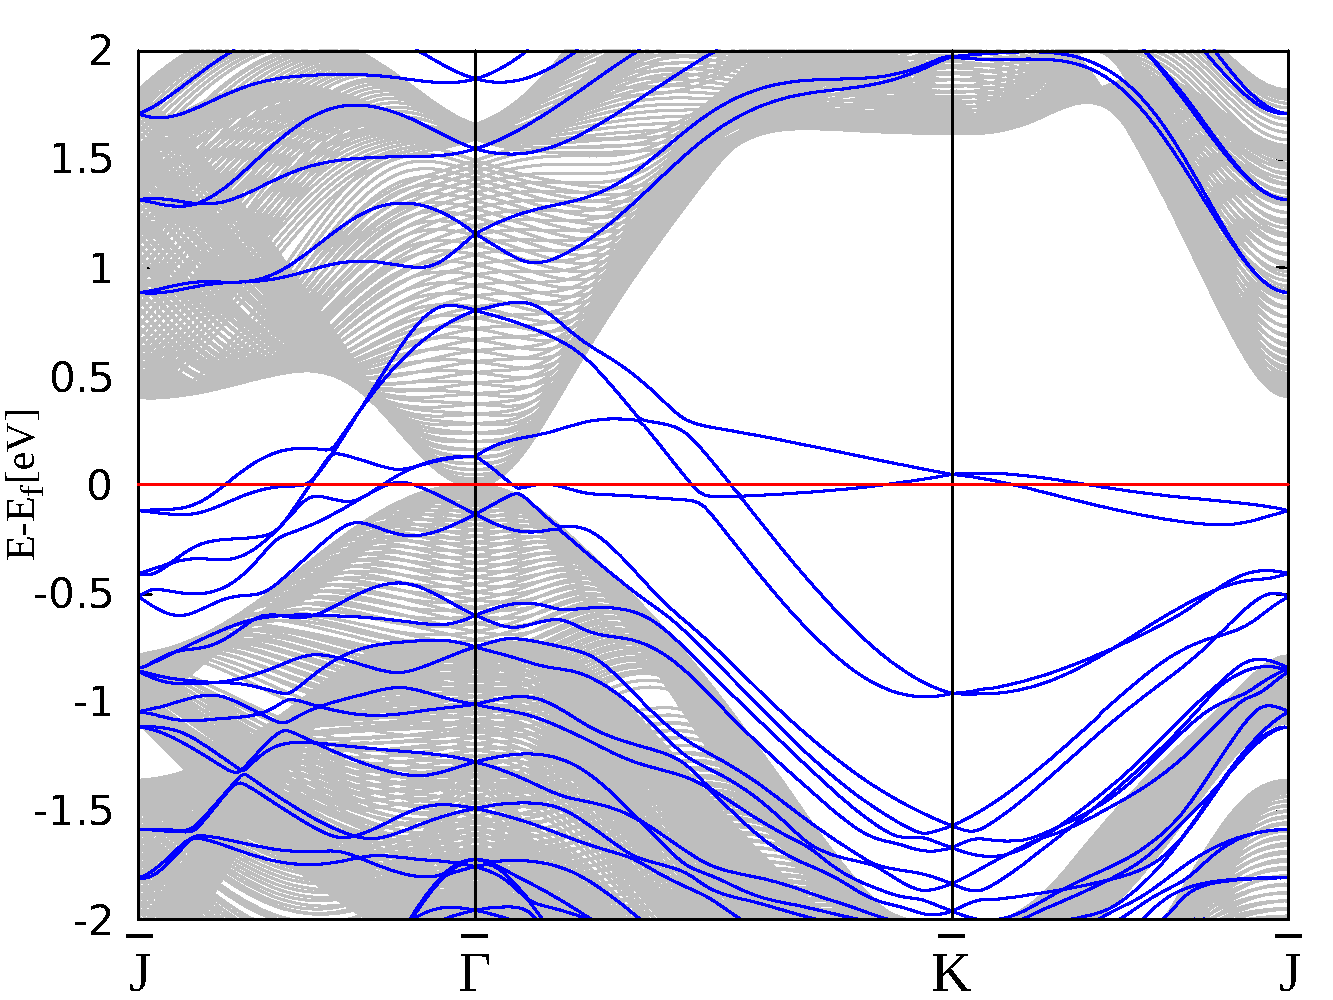
\includegraphics[width=\linewidth]{Hg_termination/bulk+9_layers_no_dos_-2_2.pdf}
%			\caption{9 layers with hydrogens on the bottom passivating one of the Hg surface terminations}
		\end{column}
	\end{columns}
	\vspace{.3cm}
	\footnotesize{
		First row: without hydrogens. \\Second row: with hydrogens passivating one surface.}
\end{frame}

\begin{frame}{PBBS with 16 and 17 layer slabs}
	\begin{columns}
		\begin{column}{.34\linewidth}
			\centering
			Te-Hg termination
		\end{column}
		\begin{column}{.34\linewidth}
			\centering
			Te-Te termination
		\end{column}
		\begin{column}{.34\linewidth}
			\centering
			Hg-Hg termination
		\end{column}
	\end{columns}
	\begin{columns}
		\begin{column}{.34\linewidth}
			\centering 
			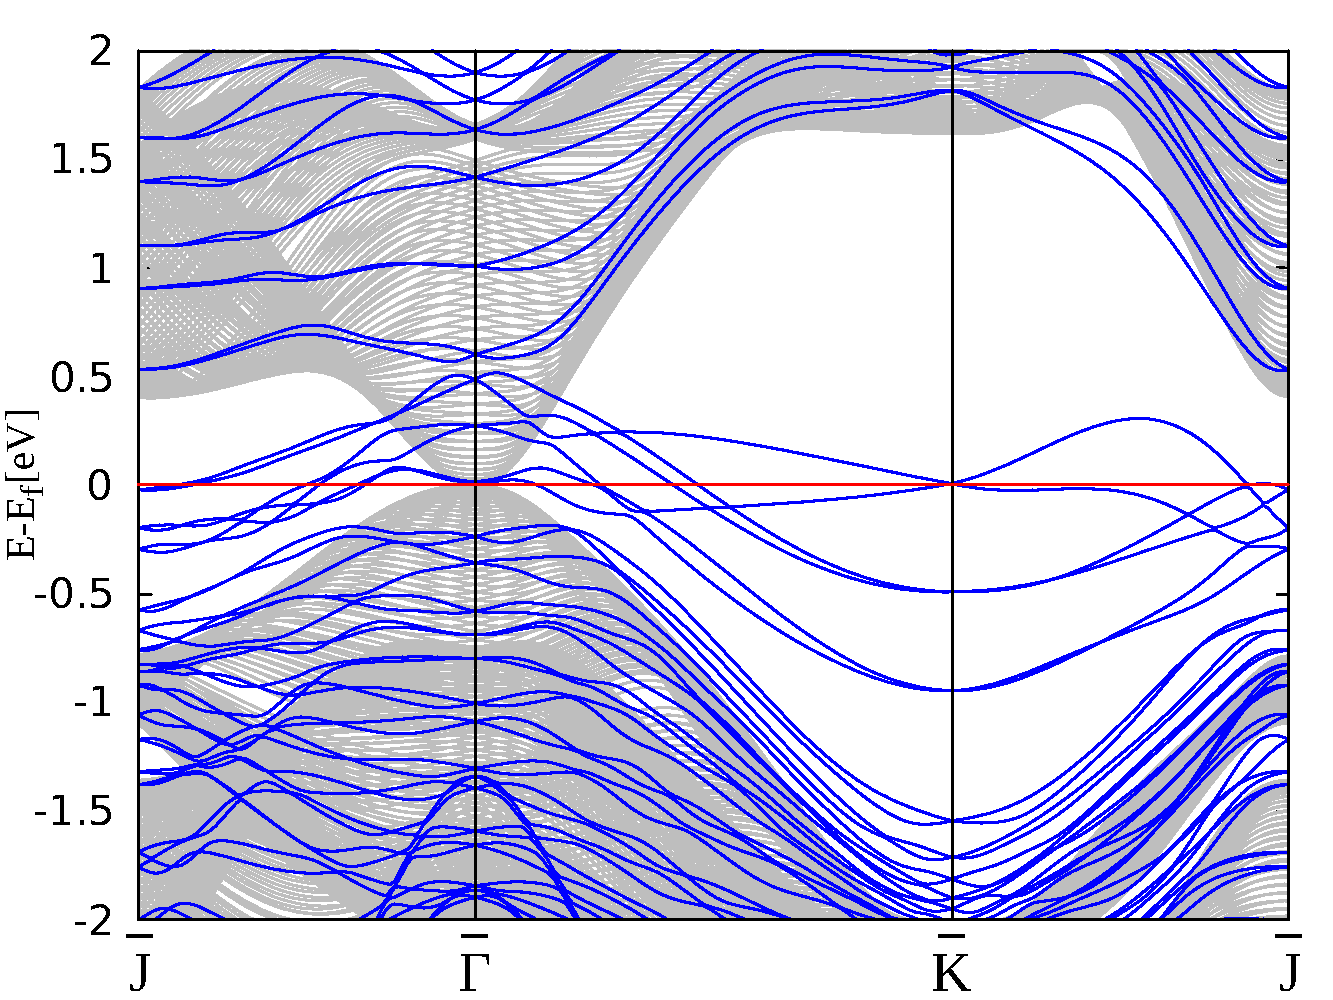
\includegraphics[width=\linewidth]{Te_and_Hg_termination/no_H_bulk+16_layers_no_dos_-2_2.pdf}
%			\caption{16 layers without hydrogens passivating the Te termination} \label{}
		\end{column}
		\begin{column}{.34\linewidth}
			\centering 
			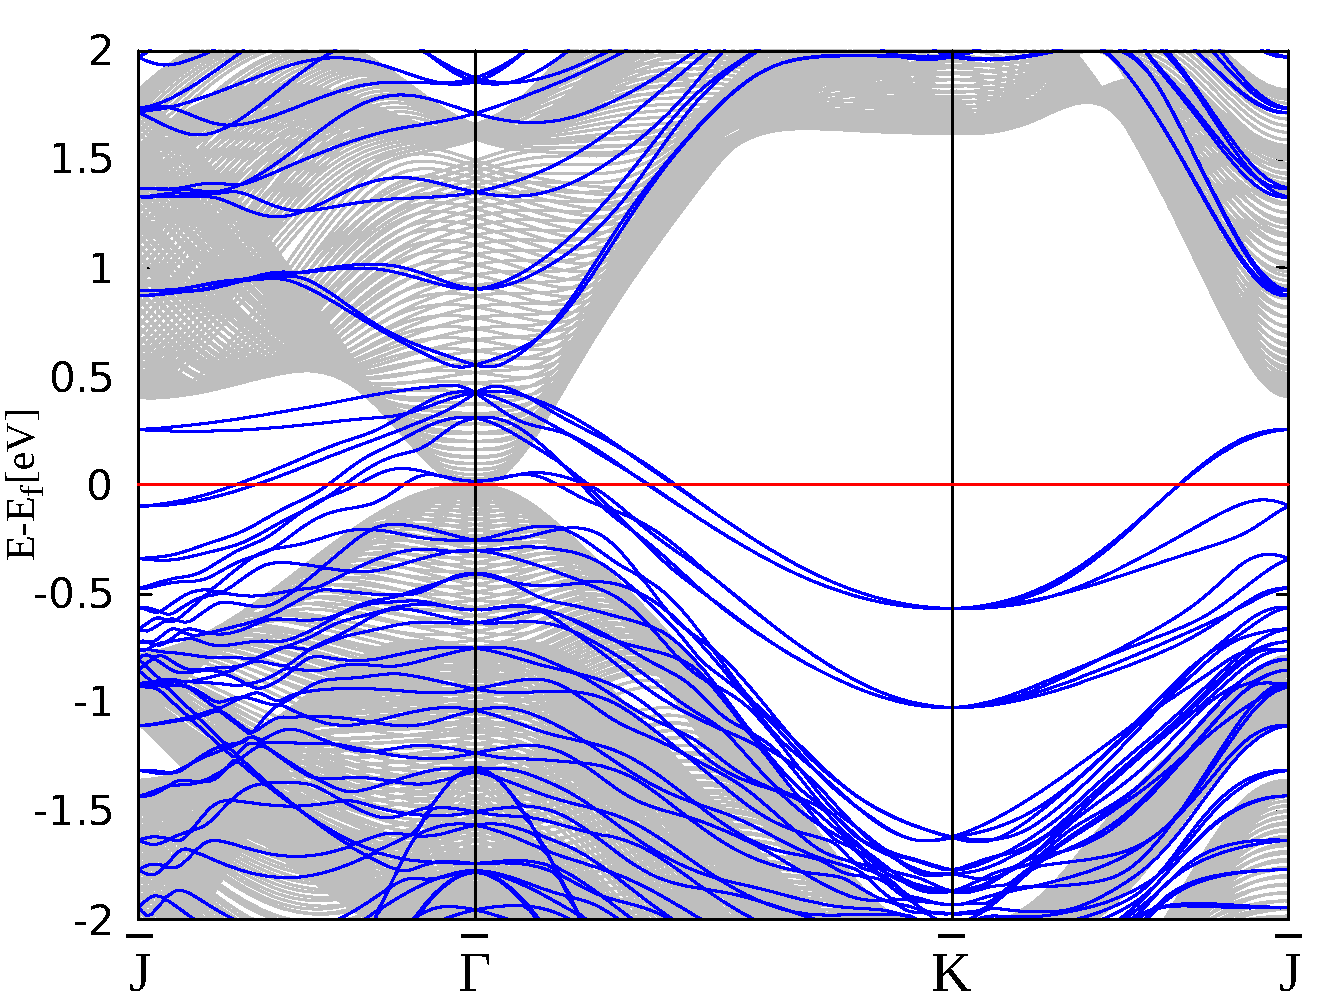
\includegraphics[width=\linewidth]{Te_termination/no_H_bulk+17_layers_no_dos_-2_2.pdf}
%			\caption{17 layers without hydrogens passivating one of the surfaces} 
		\end{column}
		\begin{column}{.34\linewidth}
			\centering 
			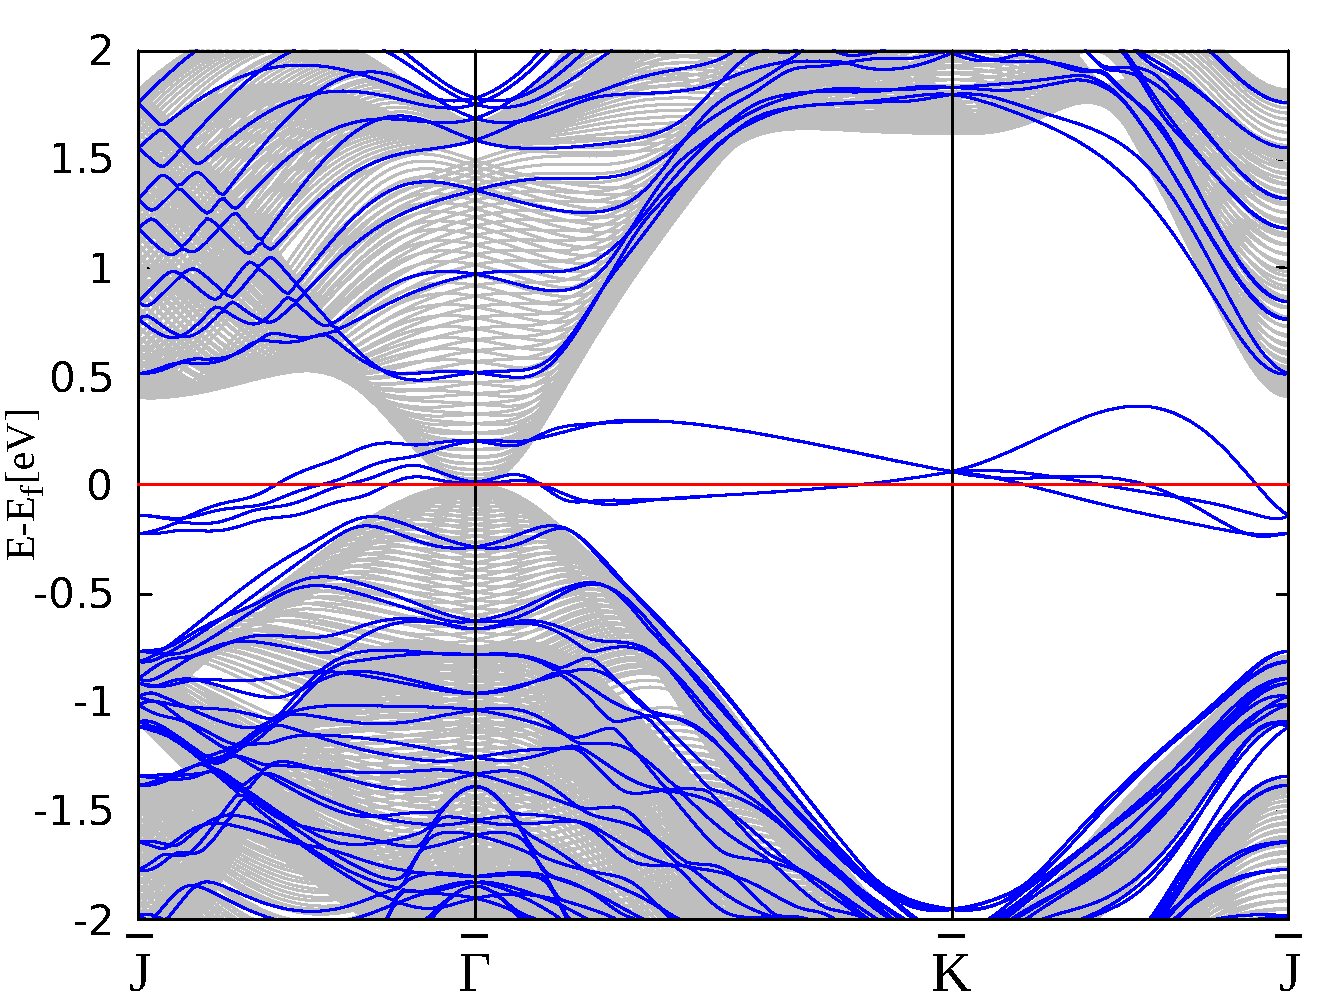
\includegraphics[width=\linewidth]{Hg_termination/no_H_bulk+17_layers_no_dos_-2_2.pdf}
%			\caption{17 layers without hydrogens passivating one of the surfaces} \label{}
		\end{column}
	\end{columns}
	\begin{columns}
		\begin{column}{.34\linewidth}
			\centering
			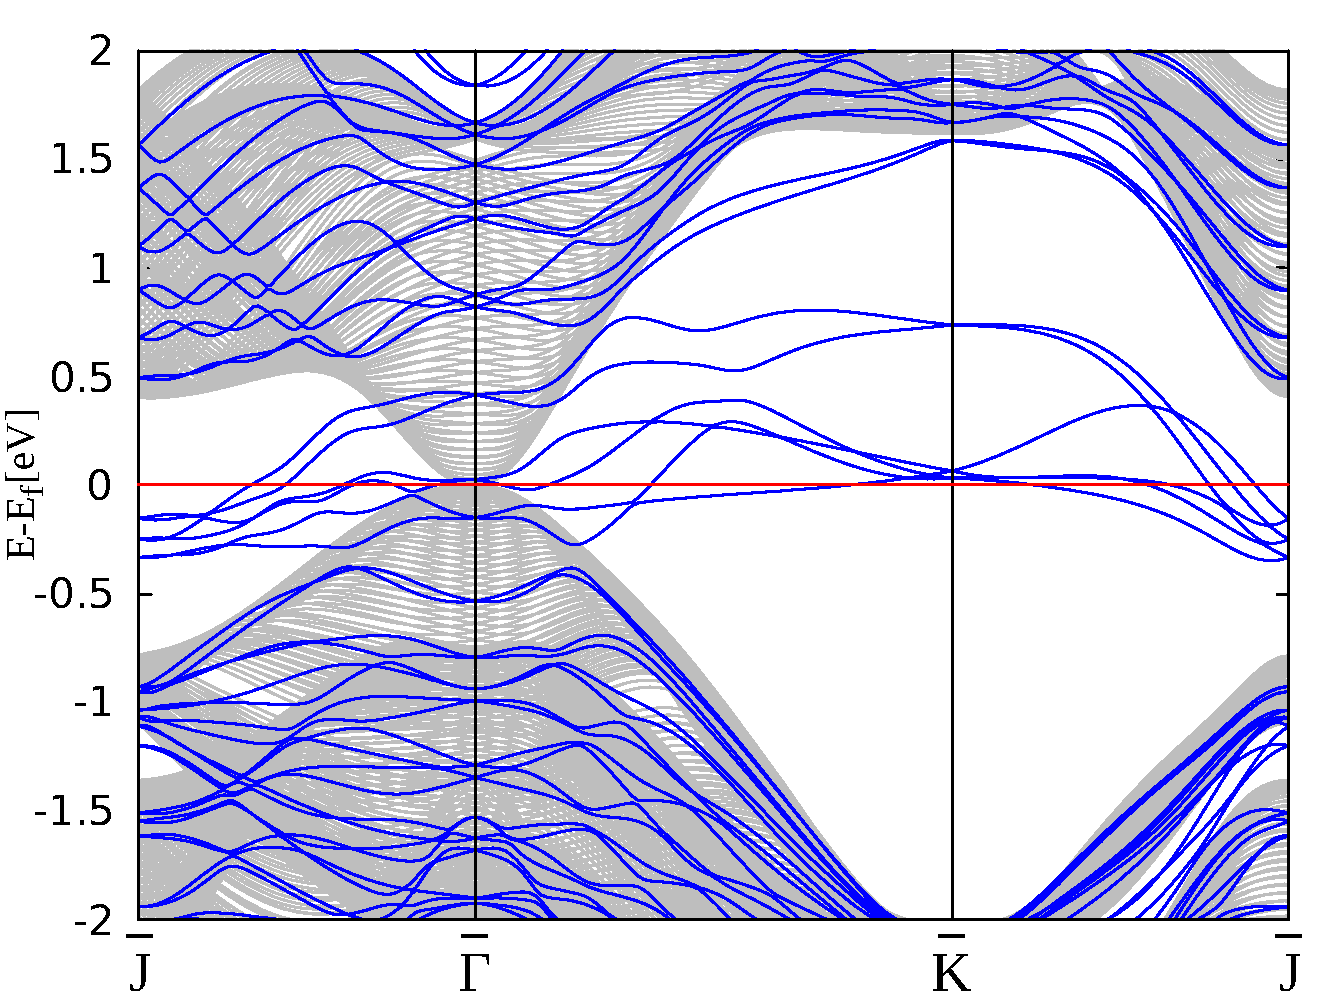
\includegraphics[width=\linewidth]{Te_and_Hg_termination/bulk+16_layers_no_dos_-2_2.pdf}
%			\caption{16 layers with hydrogens on the bottom passivating the Te surface terminations}
		\end{column}
		\begin{column}{.34\linewidth}
			\centering
			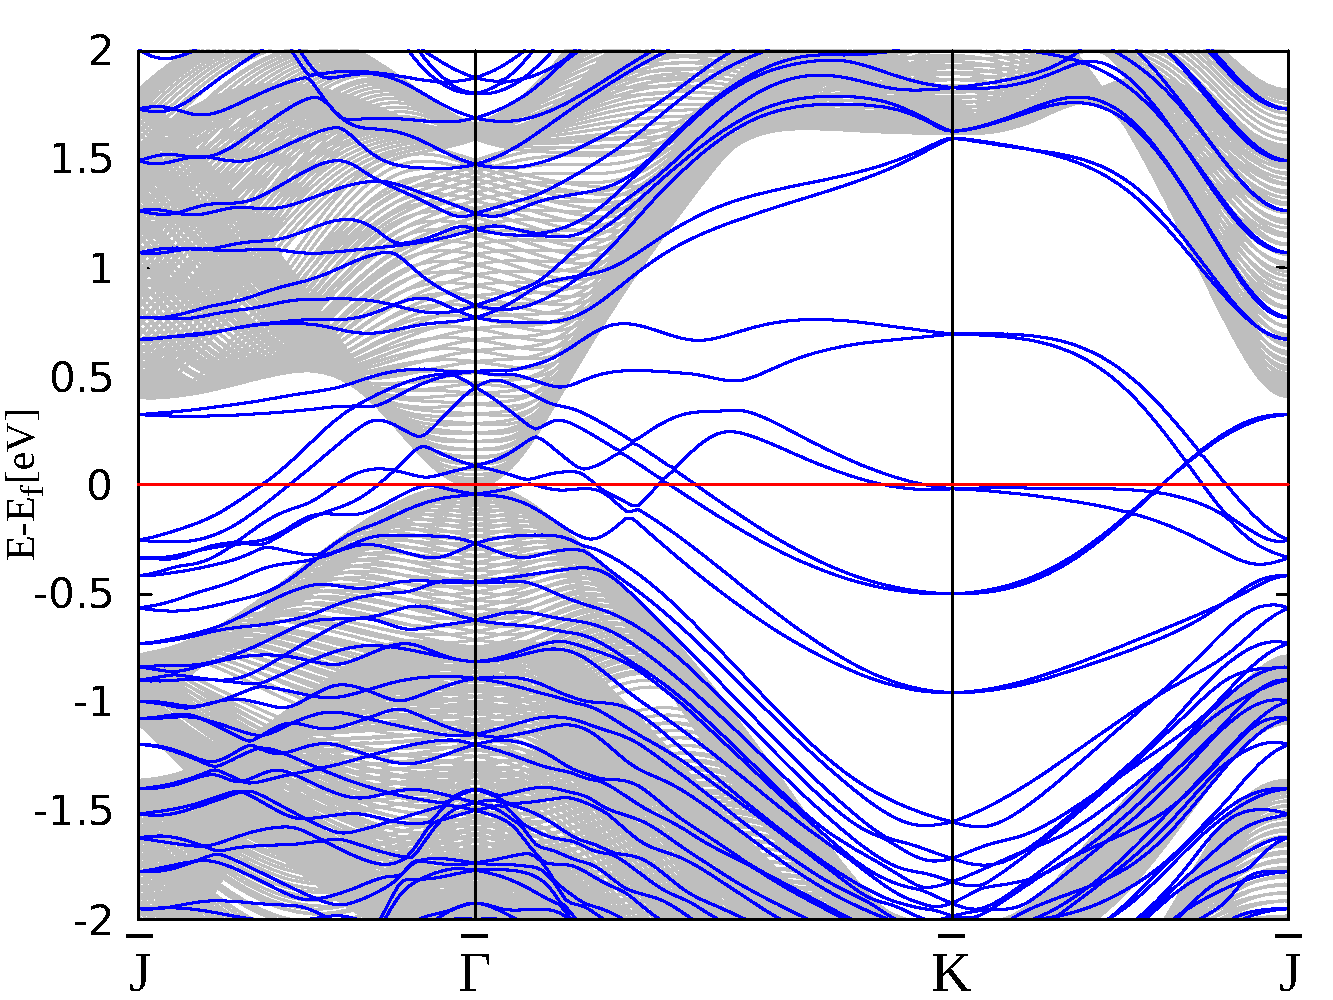
\includegraphics[width=\linewidth]{Te_termination/bulk+17_layers_no_dos_-2_2.pdf}
%			\caption{17 layers with hydrogens on the bottom passivating one of the Te surface terminations}
		\end{column}
		\begin{column}{.34\linewidth}
			\centering
			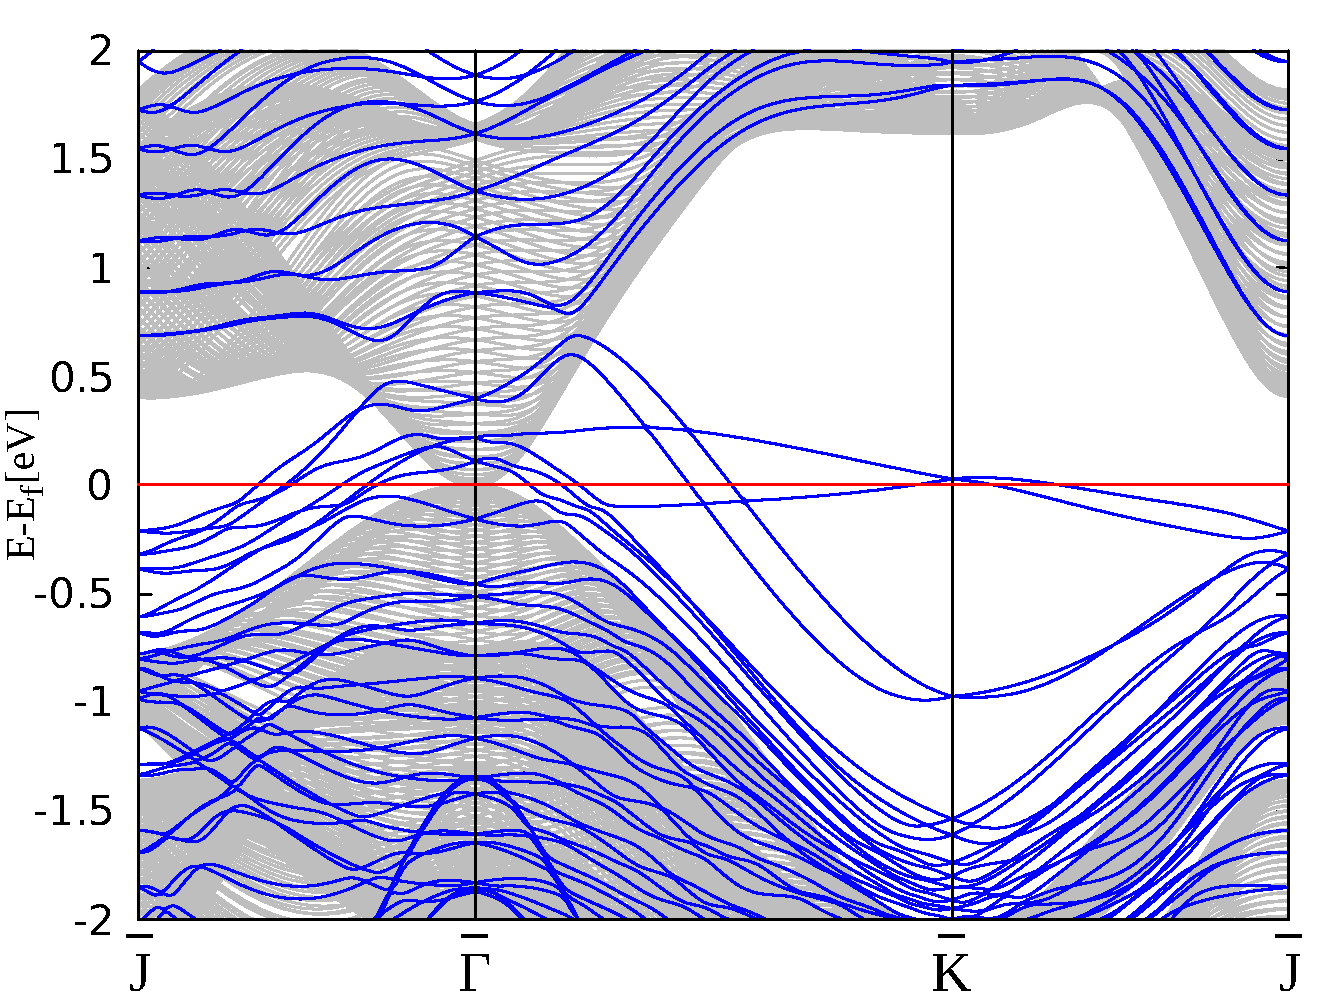
\includegraphics[width=\linewidth]{Hg_termination/bulk+17_layers_no_dos_-2_2.pdf}
%			\caption{17 layers with hydrogens on the bottom passivating one of the Hg surface terminations}
		\end{column}
	\end{columns}
	\vspace{.3cm}
	\footnotesize{
		First row: without hydrogens. \\Second row: with hydrogens passivating one surface.}
\end{frame}

%%% Local Variables:
%%% mode: latex
%%% TeX-master: "main_BA2_Vortrag.tex"
%%% End:
	
	\section{Conclusion}
	\begin{frame}{Conclusion}
	blub2
\end{frame}
%%% Local Variables:
%%% mode: latex
%%% TeX-master: "main_BA2_Vortrag.tex"
%%% End:
	
\end{document}

%%% Local Variables:
%%% mode: latex
%%% TeX-master: "main_BA2_Vortrag.tex"
%%% End: